%%% Hlavní soubor. Zde se definují základní parametry a odkazuje se na ostatní části. %%%

%% Verze pro jednostranný tisk:
% Okraje: levý 40mm, pravý 25mm, horní a dolní 25mm
% (ale pozor, LaTeX si sám přidává 1in)
\documentclass[12pt,a4paper]{report}
\setlength\textwidth{145mm}
\setlength\textheight{247mm}
\setlength\oddsidemargin{15mm}
\setlength\evensidemargin{15mm}
\setlength\topmargin{0mm}
\setlength\headsep{0mm}
\setlength\headheight{0mm}
% \openright zařídí, aby následující text začínal na pravé straně knihy
\let\openright=\clearpage

%% Pokud tiskneme oboustranně:
% \documentclass[12pt,a4paper,twoside,openright]{report}
% \setlength\textwidth{145mm}
% \setlength\textheight{247mm}
% \setlength\oddsidemargin{14.2mm}
% \setlength\evensidemargin{0mm}
% \setlength\topmargin{0mm}
% \setlength\headsep{0mm}
% \setlength\headheight{0mm}
% \let\openright=\cleardoublepage

%% Vytváříme PDF/A-2u
\usepackage[a-2u]{pdfx}

%% Přepneme na českou sazbu a fonty Latin Modern
\usepackage[czech]{babel}
\usepackage{lmodern}
\usepackage[T1]{fontenc}
\usepackage{textcomp}

%% Použité kódování znaků: obvykle latin2, cp1250 nebo utf8:
\usepackage[utf8]{inputenc}

%%% Další užitečné balíčky (jsou součástí běžných distribucí LaTeXu)
\usepackage{amsmath}        % rozšíření pro sazbu matematiky
\usepackage{amsfonts}       % matematické fonty
\usepackage{amsthm}         % sazba vět, definic apod.
\usepackage{bbding}         % balíček s nejrůznějšími symboly
			    % (čtverečky, hvězdičky, tužtičky, nůžtičky, ...)
\usepackage{bm}             % tučné symboly (příkaz \bm)
\usepackage{graphicx}       % vkládání obrázků
\usepackage{fancyvrb}       % vylepšené prostředí pro strojové písmo
\usepackage{indentfirst}    % zavede odsazení 1. odstavce kapitoly
\usepackage[square,numbers]{natbib}         % zajištuje možnost odkazovat na literaturu
			    % stylem AUTOR (ROK), resp. AUTOR [ČÍSLO]
\usepackage[nottoc]{tocbibind} % zajistí přidání seznamu literatury,
                            % obrázků a tabulek do obsahu
\usepackage{icomma}         % inteligetní čárka v matematickém módu
\usepackage{dcolumn}        % lepší zarovnání sloupců v tabulkách
\usepackage{booktabs}       % lepší vodorovné linky v tabulkách
\usepackage{paralist}       % lepší enumerate a itemize
\usepackage{xcolor}         % barevná sazba

%%% Údaje o práci

% Název práce v jazyce práce (přesně podle zadání)
\def\NazevPrace{Webový plugin pro vizualizaci sady sekundárních struktur RNA}

% Název práce v angličtině
\def\NazevPraceEN{Web plugin for multiple RNA secondary structure visualization}

% Jméno autora
\def\AutorPrace{Michal Hercík}

% Rok odevzdání
\def\RokOdevzdani{2023}

% Název katedry nebo ústavu, kde byla práce oficiálně zadána
% (dle Organizační struktury MFF UK, případně plný název pracoviště mimo MFF)
\def\Katedra{Katedra softwarového inženýrství}
\def\KatedraEN{Department of Software Engineering}

% Jedná se o katedru (department) nebo o ústav (institute)?
\def\TypPracoviste{Katedra}
\def\TypPracovisteEN{Department}

% Vedoucí práce: Jméno a příjmení s~tituly
\def\Vedouci{doc. RNDr. David Hoksza, Ph.D.}

% Pracoviště vedoucího (opět dle Organizační struktury MFF)
\def\KatedraVedouciho{Katedra softwarového inženýrství}
\def\KatedraVedoucihoEN{Department of Software Engineering}

% Studijní program a obor
\def\StudijniProgram{Informatika}
\def\StudijniObor{Programování a vývoj software}

% Nepovinné poděkování (vedoucímu práce, konzultantovi, tomu, kdo
% zapůjčil software, literaturu apod.)
\def\Podekovani{%
TODO: podekovani
}

% Abstrakt (doporučený rozsah cca 80-200 slov; nejedná se o zadání práce)
\def\Abstrakt{%
TODO
}
\def\AbstraktEN{%
TODO
}

% 3 až 5 klíčových slov (doporučeno), každé uzavřeno ve složených závorkách
\def\KlicovaSlova{%
{bioinformatika} {RNA} {sekundární struktura} {web} {plugin}
}
\def\KlicovaSlovaEN{%
{bioinformatics} {RNA} {secondary structure} {web} {plugin}
}

%% Balíček hyperref, kterým jdou vyrábět klikací odkazy v PDF,
%% ale hlavně ho používáme k uložení metadat do PDF (včetně obsahu).
%% Většinu nastavítek přednastaví balíček pdfx.
\hypersetup{unicode}
\hypersetup{breaklinks=true}

%% Definice různých užitečných maker (viz popis uvnitř souboru)
%%% Tento soubor obsahuje definice různých užitečných maker a prostředí %%%
%%% Další makra připisujte sem, ať nepřekáží v ostatních souborech.     %%%

%%% Drobné úpravy stylu

% Tato makra přesvědčují mírně ošklivým trikem LaTeX, aby hlavičky kapitol
% sázel příčetněji a nevynechával nad nimi spoustu místa. Směle ignorujte.
\makeatletter
\def\@makechapterhead#1{
  {\parindent \z@ \raggedright \normalfont
   \Huge\bfseries \thechapter. #1
   \par\nobreak
   \vskip 20\p@
}}
\def\@makeschapterhead#1{
  {\parindent \z@ \raggedright \normalfont
   \Huge\bfseries #1
   \par\nobreak
   \vskip 20\p@
}}
\makeatother

% Toto makro definuje kapitolu, která není očíslovaná, ale je uvedena v obsahu.
\def\chapwithtoc#1{
\chapter*{#1}
\addcontentsline{toc}{chapter}{#1}
}

% Trochu volnější nastavení dělení slov, než je default.
\lefthyphenmin=2
\righthyphenmin=2

% Zapne černé "slimáky" na koncích řádků, které přetekly, abychom si
% jich lépe všimli.
% \overfullrule=1mm

%%% Makra pro definice, věty, tvrzení, příklady, ... (vyžaduje baliček amsthm)

\theoremstyle{plain}
\newtheorem{veta}{Věta}
\newtheorem{lemma}[veta]{Lemma}
\newtheorem{tvrz}[veta]{Tvrzení}

\theoremstyle{plain}
\newtheorem{definice}{Definice}

\theoremstyle{remark}
\newtheorem*{dusl}{Důsledek}
\newtheorem*{pozn}{Poznámka}
\newtheorem*{prikl}{Příklad}

%%% Prostředí pro důkazy

\newenvironment{dukaz}{
  \par\medskip\noindent
  \textit{Důkaz}.
}{
\newline
\rightline{$\qedsymbol$}
}

%%% Prostředí pro sazbu kódu, případně vstupu/výstupu počítačových
%%% programů. (Vyžaduje balíček fancyvrb -- fancy verbatim.)

\DefineVerbatimEnvironment{code}{Verbatim}{fontsize=\small, frame=single}

%%% Prostor reálných, resp. přirozených čísel
\newcommand{\R}{\mathbb{R}}
\newcommand{\N}{\mathbb{N}}

%%% Užitečné operátory pro statistiku a pravděpodobnost
\DeclareMathOperator{\pr}{\textsf{P}}
\DeclareMathOperator{\E}{\textsf{E}\,}
\DeclareMathOperator{\var}{\textrm{var}}
\DeclareMathOperator{\sd}{\textrm{sd}}

%%% Příkaz pro transpozici vektoru/matice
\newcommand{\T}[1]{#1^\top}

%%% Vychytávky pro matematiku
\newcommand{\goto}{\rightarrow}
\newcommand{\gotop}{\stackrel{P}{\longrightarrow}}
\newcommand{\maon}[1]{o(n^{#1})}
\newcommand{\abs}[1]{\left|{#1}\right|}
\newcommand{\dint}{\int_0^\tau\!\!\int_0^\tau}
\newcommand{\isqr}[1]{\frac{1}{\sqrt{#1}}}

%%% Vychytávky pro tabulky
\newcommand{\pulrad}[1]{\raisebox{1.5ex}[0pt]{#1}}
\newcommand{\mc}[1]{\multicolumn{1}{c}{#1}}

%%% Pro generovany tex pomocí pandoc
\providecommand{\tightlist}{%
  \setlength{\itemsep}{0pt}\setlength{\parskip}{0pt}}


%% Titulní strana a různé povinné informační strany
\begin{document}
%%% Titulní strana práce a další povinné informační strany

%%% Titulní strana práce

\pagestyle{empty}
\hypersetup{pageanchor=false}

\begin{center}

\centerline{\mbox{
\includegraphics[width=166mm]{../img/logo-cs.pdf}}}

\vspace{-8mm}
\vfill

{\bf\Large BAKALÁŘSKÁ PRÁCE}

\vfill

{\LARGE\AutorPrace}

\vspace{15mm}

{\LARGE\bfseries\NazevPrace}

\vfill

\Katedra

\vfill

{
\centerline{\vbox{\halign{\hbox to 0.45\hsize{\hfil #}&\hskip 0.5em\parbox[t]{0.45\hsize}{\raggedright #}\cr
Vedoucí bakalářské práce:&\Vedouci \cr
\noalign{\vspace{2mm}}
Studijní program:&\StudijniProgram \cr
\noalign{\vspace{2mm}}
Studijní obor:&\StudijniObor \cr
}}}}

\vfill

% Zde doplňte rok
Praha \RokOdevzdani

\end{center}

\newpage

%%% Následuje vevázaný list -- kopie podepsaného "Zadání bakalářské práce".
%%% Toto zadání NENÍ součástí elektronické verze práce, nescanovat.

%%% Strana s čestným prohlášením k bakalářské práci

\openright
\hypersetup{pageanchor=true}
\pagestyle{plain}
\pagenumbering{roman}
\vglue 0pt plus 1fill

\noindent
Prohlašuji, že jsem tuto bakalářskou práci vypracoval(a) samostatně a výhradně
s~použitím citovaných pramenů, literatury a dalších odborných zdrojů.
Tato práce nebyla využita k získání jiného nebo stejného titulu.

\medskip\noindent
Beru na~vědomí, že se na moji práci vztahují práva a povinnosti vyplývající
ze zákona č. 121/2000 Sb., autorského zákona v~platném znění, zejména skutečnost,
že Univerzita Karlova má právo na~uzavření licenční smlouvy o~užití této
práce jako školního díla podle §60 odst. 1 autorského zákona.

\vspace{10mm}

\hbox{\hbox to 0.5\hsize{%
V \hbox to 6em{\dotfill} dne \hbox to 6em{\dotfill}
\hss}\hbox to 0.5\hsize{\dotfill\quad}}
\smallskip
\hbox{\hbox to 0.5\hsize{}\hbox to 0.5\hsize{\hfil Podpis autora\hfil}}

\vspace{20mm}
\newpage

%%% Poděkování

\openright

\noindent
\Podekovani

\newpage

%%% Povinná informační strana bakalářské práce

\openright

\vbox to 0.5\vsize{
\setlength\parindent{0mm}
\setlength\parskip{5mm}

Název práce:
\NazevPrace

Autor:
\AutorPrace

\TypPracoviste:
\Katedra

Vedoucí bakalářské práce:
\Vedouci, \KatedraVedouciho

Abstrakt:
\Abstrakt

Klíčová slova:
\KlicovaSlova

\vss}\nobreak\vbox to 0.49\vsize{
\setlength\parindent{0mm}
\setlength\parskip{5mm}

Title:
\NazevPraceEN

Author:
\AutorPrace

\TypPracovisteEN:
\KatedraEN

Supervisor:
\Vedouci, \KatedraVedoucihoEN

Abstract:
\AbstraktEN

Keywords:
\KlicovaSlovaEN

\vss}

\newpage

\openright
\pagestyle{plain}
\pagenumbering{arabic}
\setcounter{page}{1}


%%% Strana s automaticky generovaným obsahem bakalářské práce

\tableofcontents

%%% Jednotlivé kapitoly práce jsou pro přehlednost uloženy v samostatných souborech
\chapter*{Úvod}
\addcontentsline{toc}{chapter}{Úvod}

RNA má více funkcí než pouze přenos genetické informace. Zkoumání struktur RNA
napříč různými živočišnými druhy a sledování podobností, které mohou hrát
důležitou roli v její funkci, může vést k lepšímu pochopení
evoluce\cite{kyticky} nebo některých nemocí\cite{disease}, speciálně se zkoumá
například v souvislosti s rakovinou\cite{cancer, cancer2} nebo neurologickými
onemocněními\cite{neuro, neuro2}.

Funkce RNA je odvozená od její 3D struktury (terciární struktury) a ačkoliv
její predikce je aktivně zkoumané téma\cite{3DStructure1, 3DStructure2}, je
stále těžké jí získat. Mnohem více známé jsou sekundární struktury. Ty o
prostorovém rozložení říkají pouze to, že spárované nukleotidy jsou blízko
sebe, ale přesto nabízí dobrý popis.

Pro analýzu sekundárních struktur RNA existuje mnoho nástrojů. Nástroje se
typicky soustředí na možnosti anotace, editace nebo porovnávání omezeného
množství sekundárních struktur RNA a neexistuje nástroj, který by umožňoval
interaktivně porovnávat mezi sebou libovolné množství sekundárních struktur
RNA. Většina nástrojů navíc nenabízí možnost integrace do jiných programů,
například do webových databází sekundárních struktur.

Z těchto důvodů představujeme knihovnu napsanou v jazyce Typescript, která
umožňuje jednoduše vizualizovat sekundární struktury a nabízí metody pro
porovnávaní podobných struktur, které můžou hrát klíčovou roli k pochopení
biologických mechanismů.


\chapter{Úvod do problematiky}

\section {Seznámení s biologickými pojmy}

\subsection{RNA} 

{\color{red}Rozdělit do více kapitol. Jedna z kapitol struktura RNA.}

\subsection{funkce}

RNA (zkratka z anglického ribonucleic acid) je biomolekula, která hraje
klíčovou roli v procesu přenosu genetické informace u všech živých organismů.
RNA se skládá z řetězce nukleotidů, které obsahují cukr ribózu, fosfátovou
skupinu a jednu z pěti dusíkatých bází (adenin, guanin, cytosin, uracil nebo
inosin). Existují různé typy RNA, jako jsou messenger RNA (mRNA), ribozomální
RNA (rRNA) a transfer RNA (tRNA), které mají každý svou specifickou funkci v
buňce.

RNA sekundární struktura se týká způsobu, jakým se molekula RNA skládá na sebe
díky vzniku bázových párů mezi komplementárními nukleotidy. Bázové párování se
děje mezi dusíkatými bázemi RNA nukleotidů, přičemž adenin (A) se páruje s
uracilem (U) a guanin (G) se páruje s cytosinem (C).

RNA sekundární struktura je důležitá, protože může ovlivnit to, jak RNA
molekula funguje. Například stem-loop struktura v mRNA molekule může ovlivnit
přístupnost mRNA k ribozomům, což je buněčný mechanismus zodpovědný za
překládání mRNA na proteiny.

\subsection{struktura}

\subsubsection{Hairpin loop}

\subsubsection{Bulges}

\subsubsection{multibranch loop}

\section{Vizualizace sekundárních RNA struktur} 

Pro reprezentaci sekundární RNA struktury se používají jak textové, tak
grafické způsoby. Pro nás jsou nejzajímavějsí ty grafické, ze kterých v této
části představíme tři nejpoužívanější - arc diagram, circular diagram a
radiate diagram. Obrázky ukázek diagramu v této části jsou získané za pomoci nástroje
VARNA\cite{Varna}.

V arc diagramu jsou nukleotidy zobrazeny na rovné čáře ve stejném pořadí jako v
sekvenci a bázové páry nukleotidů jsou spojeny obloukem.

\begin{figure}[H]
  \centering
  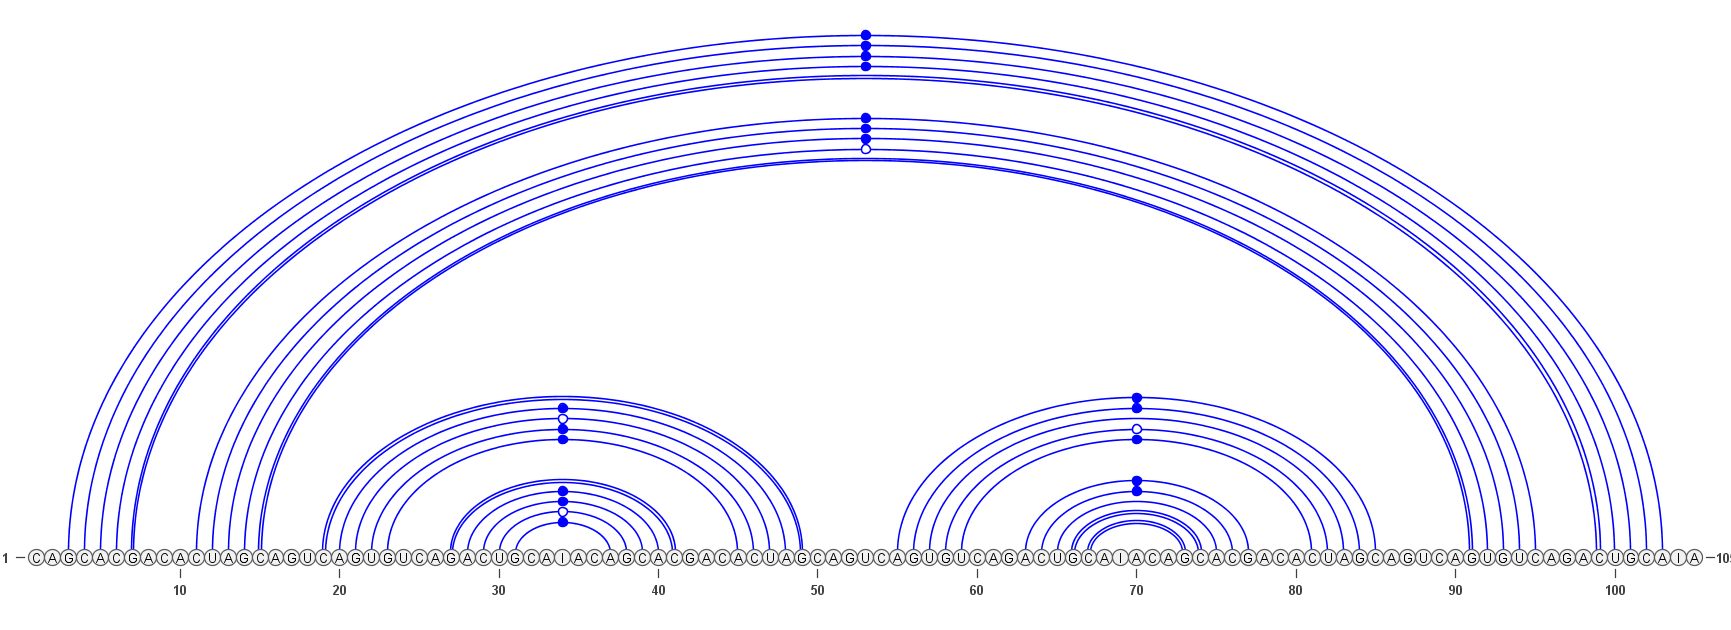
\includegraphics[width=140mm]{../img/kap01/arc.png}
  \caption{Ukázka arc diagramu}
\end{figure}

Circular diagram je velmi podobný. Nukleotidy neleží na rovné čáře, ale po
obvodu kruhu. Bázové páry jsou spojeny buď čárou nebo obloukem.

\begin{figure}[H]
  \centering
  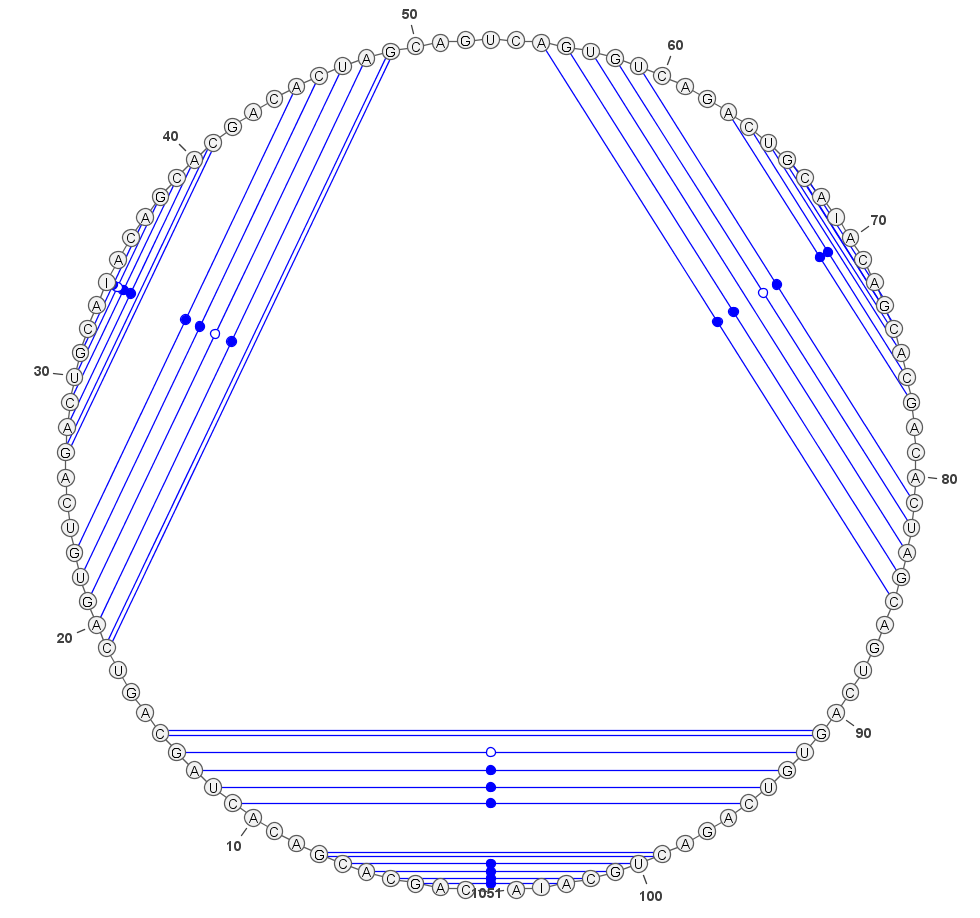
\includegraphics[height=100mm]{../img/kap01/circular.png}
  \caption{Ukázka circular diagramu}
\end{figure}

V radiate diagramu jsou pozice nukleotidů voleny tak, aby bylo možné rozeznat
motivy sekundární struktury, jako jsou hairpins, bulges nebo multibranch loops. 

\begin{figure}[H]
  \centering
  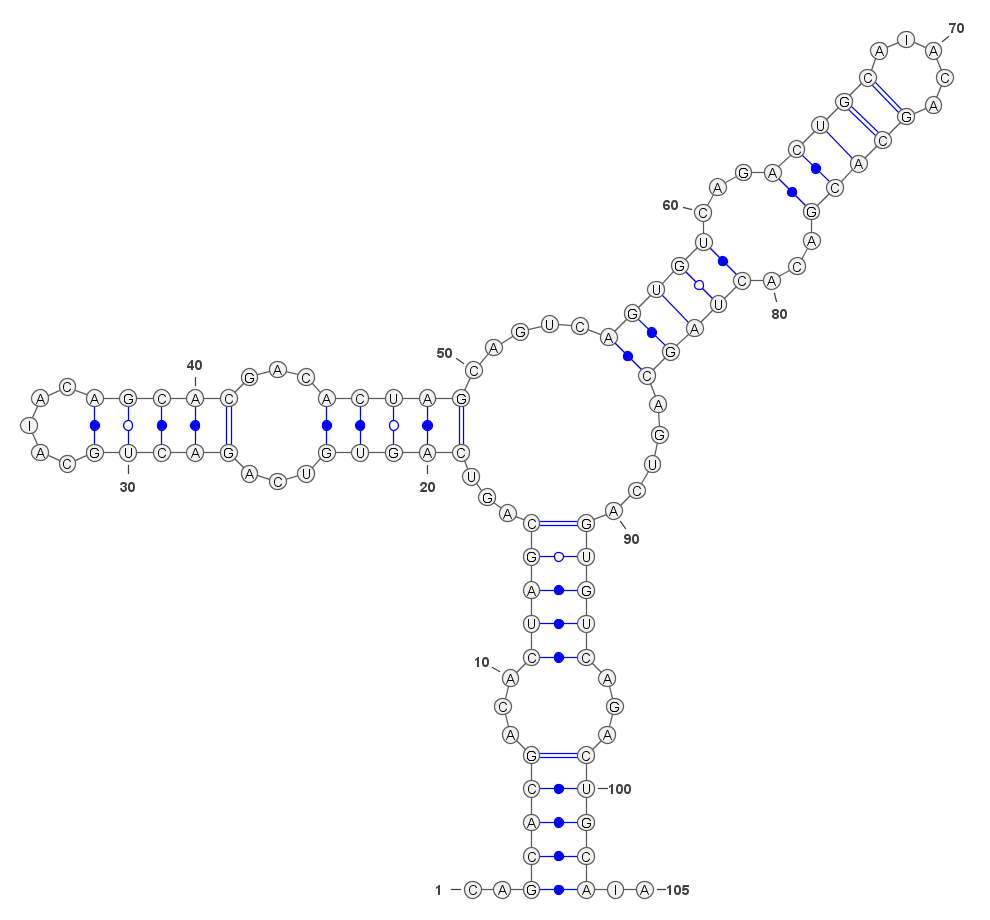
\includegraphics[height=100mm]{../img/kap01/radiate.png}
  \caption{Ukázka radiate diagramu}
\end{figure}

Právě schopnost zachytit zmíněné motivy obě předešlé reprezentace postrádají, a
proto se radiate diagram používá tam, kde je potřeba detailní vizuální analýza
motivů sekundární RNA struktury a její interakce. 


\section{Podobné projekty} {\color{red} chybi motivacni uvod, ktery by rekl, co chceme delat, aby bylo mozne pochopit podobne k cemu}

Rádi bychom čtenáře seznámili s některými nástroji, které jsou používáné pro
vizualizaci sekundárních RNA struktur. Většina z nich jsou programy s
uživatelským rozhraním a mohlo by se proto zdát zbytečné je zmiňovat nebo
porovnávat s naší knihovnou. Nicméně u níže zmíněných programů není duležité
řešení samotného uživatelského rozhraní, jako především druh zvolených metod
pro vizualizaci a následné porovnávání.

Z velkého množství existujících nástrojů, byla snaha vybrat takové,
které mají rozdílné přístupy a nabízí nejširší paletu funkcí.

\subsection{VARNA} 

VARNA (Visualization Applet for RNA) je nástroj pro automatické
kreslení, vizualizaci a anotaci sekundárních RNA struktur, navržený jako
doprovodný software pro webové servery a databáze.

VARNA implementuje algoritmy pro vykreslení všech tří výše zmíněných diagramů,
podporuje různé textové formáty pro vstup i výstup a je schopný exportovat
kresbu do rastrových nebo vektorových formátů. Umožňuje ruční úpravy a
strukturální anotace výsledku kresby a je považován za standard pro práci se
sekundárními strukturami RNA.

\begin{figure}[H]
  \centering
  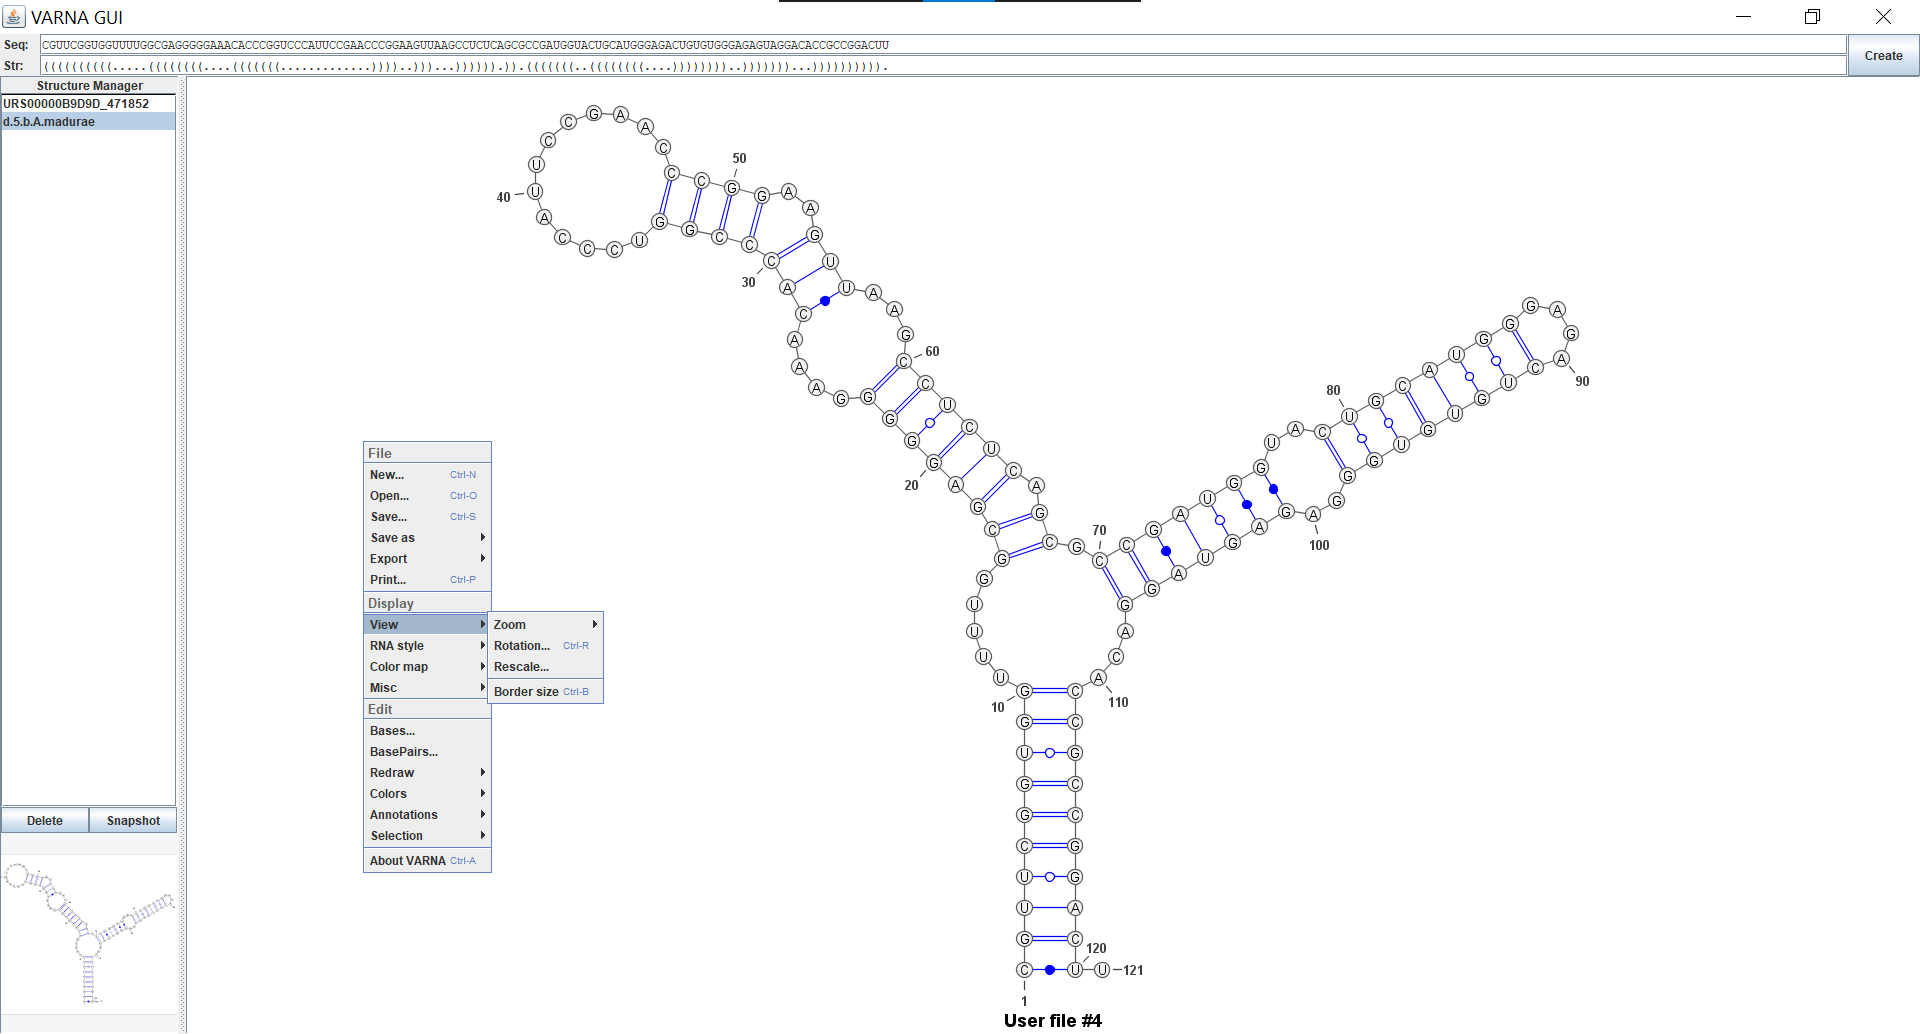
\includegraphics[width=140mm]{../img/kap01/varna.png}
  \caption{Snimek nástroje Varna. Zobrazená struktura je d.5.b.A.madurae.}
\end{figure}

\subsection{RNAStructViz} 

RNAStructViz\cite{RnaStructViz} je grafický nástroj pro analýzu sekundárních
RNA struktur. Jeho předností je vizuální porovnání tří konfigurací v circular
arc diagramu. Doplněné zabudovaným prohlížečem CT-style\footnote{CT formát
souboru slouží k ukládání informace o sekvenci a bázových párů.} souboru a
prohlížečem radial diagramu podstruktury, která je přímo propojená s arc
diagram oknem skrze nástroj pro výběr zoom. Mezi další funkce patří vypočítání
číselných informací a možnost exportu obrázků a dat pro pozdější použití.

\begin{figure}[H]
  \centering
  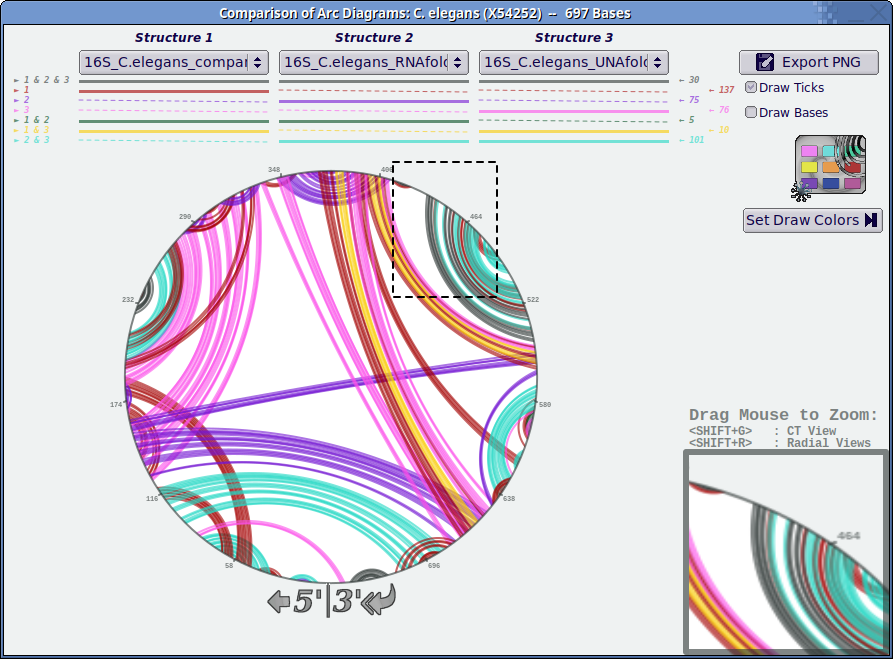
\includegraphics[width=140mm]{../img/kap01/rnaStructViz.png}
  \caption{Snimek nástroje rnaStructViz, zobrazující tři struktury RNA.}
\end{figure}

\subsection{Forna} 

Forna\cite{Forna} (force-directed rna) nabízí webové rozhraní a server, který
umožňuje uživateli vložit sekundární RNA strukturu ve formátu dot-bracket a
zobrazí ji jako force-directed
graf\footnote{https://cs.brown.edu/people/rtamassi/gdhandbook/chapters/force-directed.pdf}.
Uživatel může následně upravit pozice přetažením myší a lze i upravovat přímo
strukturu. 

\begin{figure}[H]
  \centering
  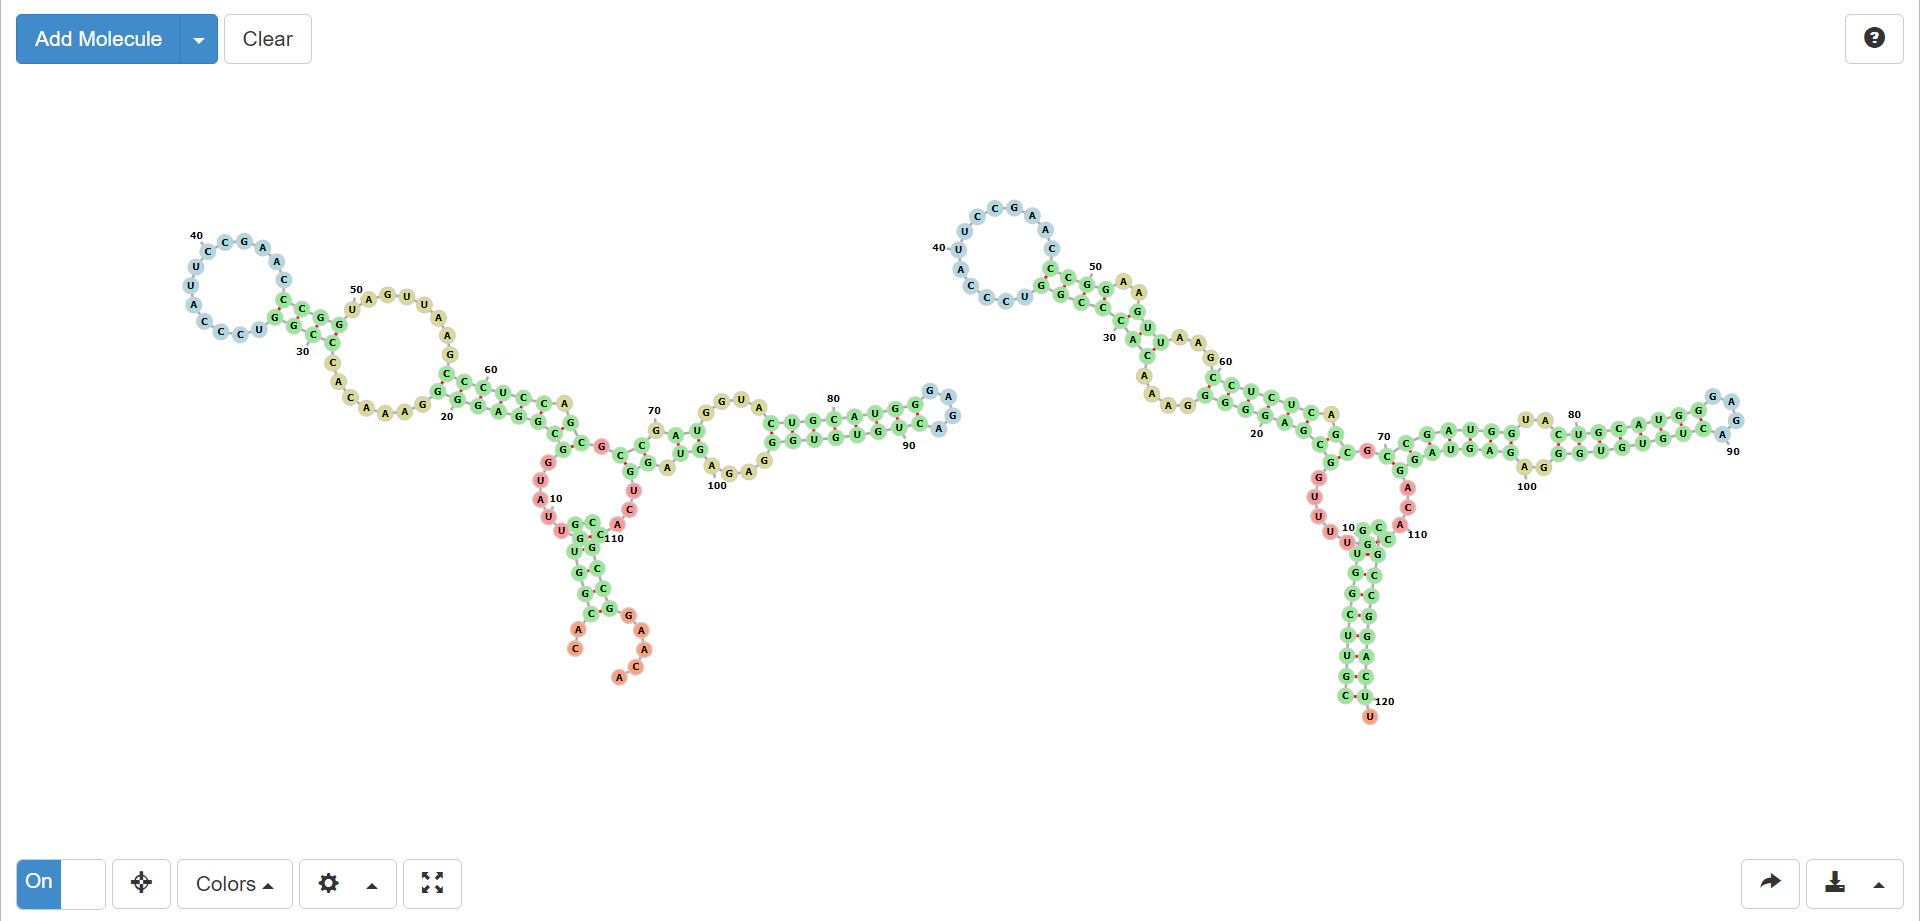
\includegraphics[width=140mm]{../img/kap01/forna.png}
  \caption{Snimek nástroje Forna. Nalevo odvozená sekundární RNA
  struktura URS00000B9D9D\_471852 od struktury d.5.b.A.madurae napravo.}
\end{figure}

\subsection{R-chie} 

R-chie \cite{Rchie} je web server, který umí vygenerovat šest různých typů arc
diagramu. Vývoj tohoto nástroje byl se zaměřením především na složitější
struktury, které nelze hezky nakreslit v radial diagramu. R-chie umí
vygenerovat diagram pro porovnávání dvou sekundárních RNA struktur. Důležitým
cílem byla možnost generovat diagramy pro velké množství dat, proto také
nenabízí grafické rozhraní a s ním spojenou interakci se strukturami. 

Projekt také nabízí balíček napsaný v jazyce
R\footnote{https://www.r-project.org/} zvaný R4RNA, který umožňuje spuštění
programu lokálně a napříč operačním systémům.

\begin{figure}[H]
  \centering
  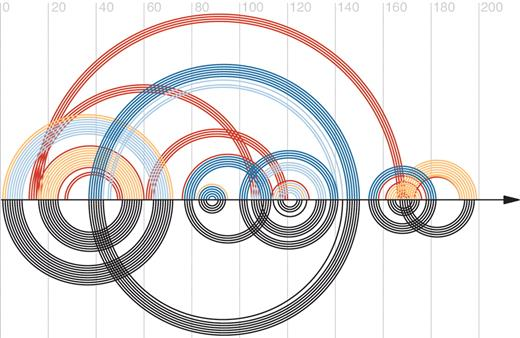
\includegraphics[width=140mm]{../img/kap01/rchie.jpeg}
  \caption{Výsledný arc diagram nástroje R-chie, zobrazující dvě sturktury.
  První struktura je nad horizontální čárou a druhá pod ní.}
\end{figure}

\subsection{Shrnutí existujících nástrojů}

Nástroje představené v této kapitole se soustředí především na prácí s circular
diagramem nebo arc diagramem, a právě pouze pro tyto diagramy nabízí nějaké
metody pro porovnávání omezeného množství sekundárních struktur RNA. Forna
podporuje pouze radial diagram, ale porovnávání dvou struktur, které sice jdou
zobrazit vedle sebe, už nijak neusnadňuje. 

Varna Podporuje všechny tři zmíněné diagrami, ale nelze ani zobrazit dvě
sekundární rna struktury vedle sebe. Velkou výhodou nástroje VARNA by byla
možnost použití na webu, ale k tomu používá Java Applets
\footnote{https://docs.oracle.com/javase/tutorial/deployment/applet/index.html},
které jsou od roku 2017 považované za zastaralé
\footnote{https://www.oracle.com/java/technologies/javase/9-deprecated-features.html}.

Ze zmíněných projektů je nejpodobnější tomu našemu R-chie, který se snaží
usnadnit porovnávání sekundárních RNA struktur a nabízí i knihovnu napsanou v
jazyce R. Liší se pak v samotném přístupu, protože jejich rozhraní generuje
pouze statické circular nebo arc diagramy.

\section{Kreslení grafů na základě šablony}

Níže jsou zmíněné dva projekty, které úzce souvisí s naší knihovnou, protože
produkují data ve formátu, se kterým pracuje naše knihovna a metody
použité ke generovaní takových dat jsou klíčové pro naší knihovnu.

\subsection{TRAVeLer} 

Traveler\cite{Traveler2017} je nástroj pro vizualizaci cílové sekundární
struktury, využívající existující rozložení dostatečně podobné RNA struktury
jako vzor. Traveler je založený na algoritmu, který konvertuje cílovou a
vzorovou strukturu do odpovídající stromové reprezentace a využije stromovou
editační vzdálenost společně s modifikací rozložení k přetvoření vzorové
struktury do cílové. Traveler přijme na vstupu sekundární strukturu a vzor
rozložení a na výstupu dá rozložení cílové struktury. Je to tedy command-line
open source nástroj schopný rychle generovat rozložení i pro největší RNA
struktury za poskytnutí dostatečně podobného rozložení.

Do vzniku Traveleru neexistoval žádný nástroj, který by dokázal velké struktury
vizualizovat ve standardni notaci, se kterou jsou biologové naučení pracovat a
porovnávat struktury napříč druhům.

\subsection{R2DT} 

R2DT\cite{R2DT2021} je metoda pro predikci a vizualizaci široké škály
sekundárních RNA struktur ve radial diagramu. R2DT je postaveno na knihovně se
3 647 vzory reprezentujícími většinu známých RNA struktur. R2DT se používá na
ncRNA\footnote{RNA, která se nepřekládá do proteinů} (non-coding RNA)
sekvencích z RNAcentral\footnote{https://rnacentral.org/} databáze a vytvořila
více než 27 miliónů diagramů\footnote{Číslo je aktuální k datu 11.4. 2023},
čímž tvoří největší světovou sadu dat s 2D RNA strukturami. Pro vizualizaci
neboli 2D rozložení používá R2DT právě výše zmíněný nástroj Traveler.


\chapter{Metody vizualizace a porovnání}

Cílem této knihovny není pouze vizualizovat sekundární strukturu RNA, ale také
usnadnit analýzu rozdílů a podobností mezi více strukturami RNA. Proto jsme se
zaměřili na práci s radial diagramy, které nejlépe zobrazujou motivy struktury
a zároveň jsou nejpřirozenější reprezentací.

Kromě toho jsme viděli potenciál generování rozložení na základě vzorové
struktury, jak to dělá nástroj Traveler. Výstupem Traveleru je soubor ve
formátu JSON, který obsahuje informace o vzoru každého nukleotidu a provedených
úpravách - přidání, odebrání, přejmenování a přesunutí nukleotidu.

Například pokud bychom použili nástroj Varna na zobrazení následujících dvou
struktur musíme všechny podobnosti vypozorovat sami. 

\begin{figure}[H]
  \centering
  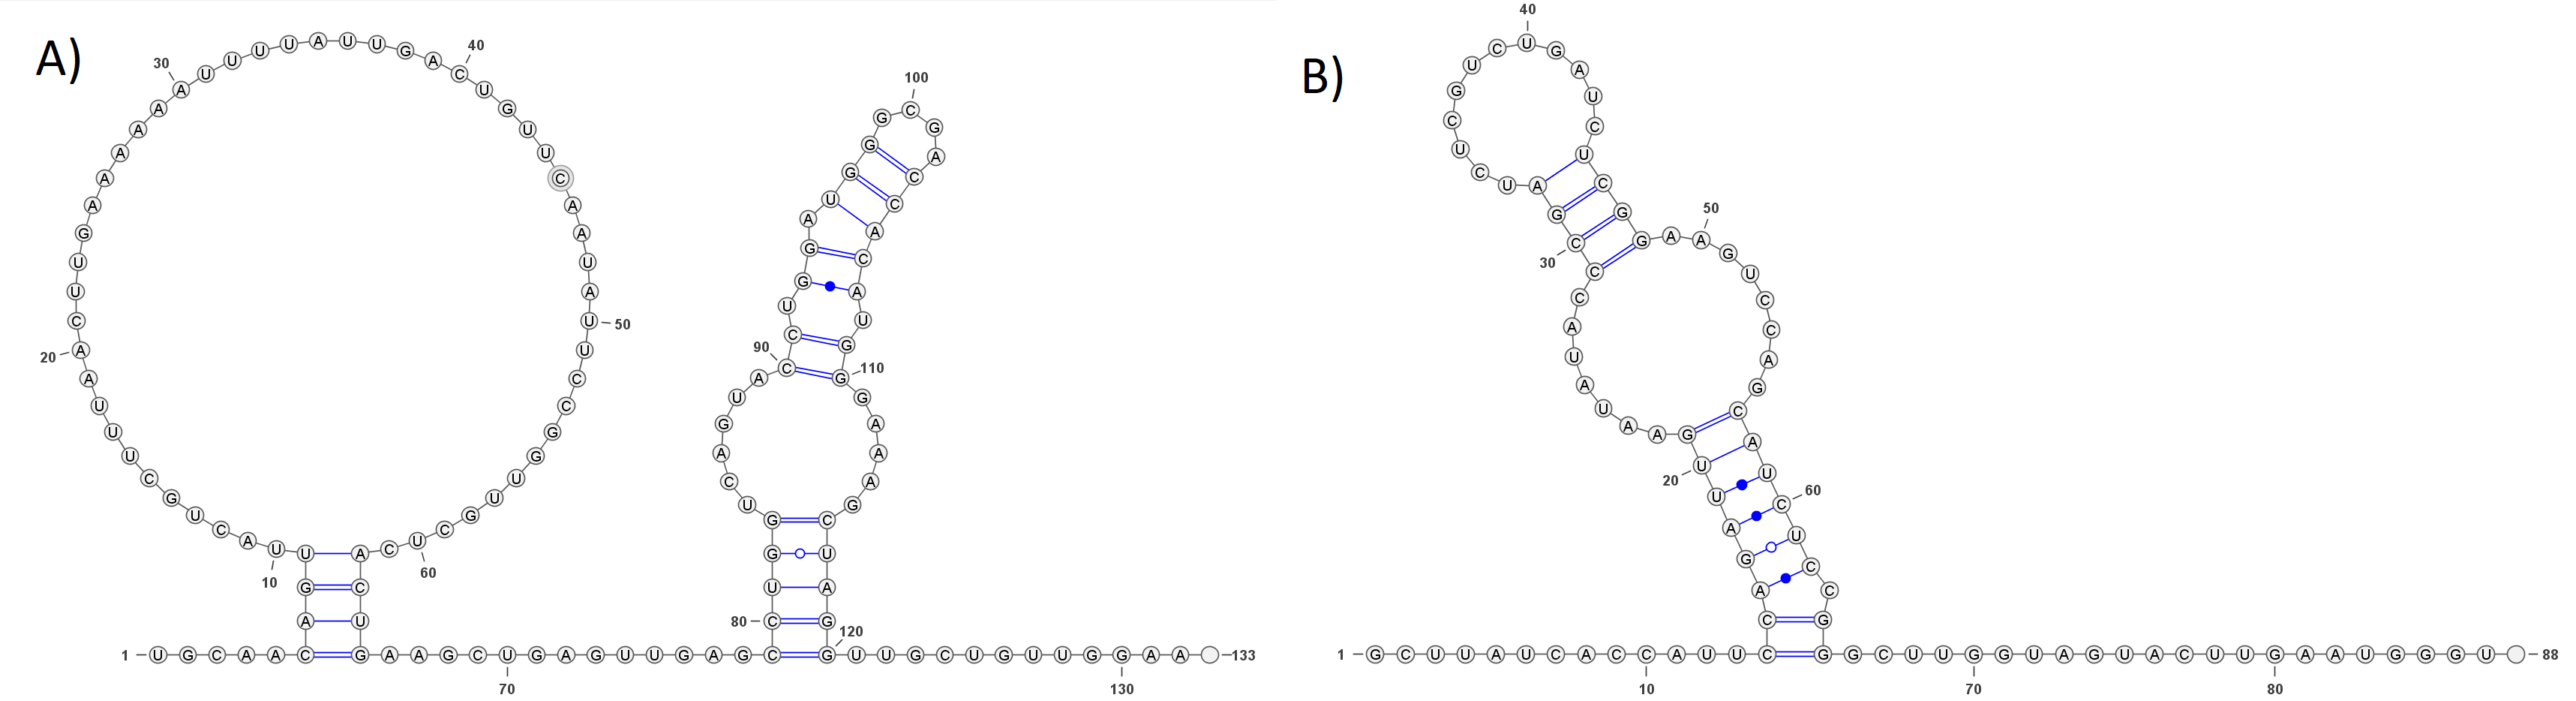
\includegraphics[width=140mm]{../img/kap02/intro/varna.png}
  \caption{Dvě sekundární RNA struktury s RNAcentral ID A) URS00006E712C, B)
  URS0000AB09C9.}
\end{figure}

Sice není těžké vypozorovat některé podobné motivy, ale není na první pohled
jasná podobnost sekvence.

Na generování obou struktur používá nástroj Traveler stejnou vzorovou
strukturu, která je v tomto konkrétním případě podobná obou odvozeným
strukturám. Podobnost odvozených struktur ke vzorové je až na vyjímky běžná, a
proto jsme se rozhodli tuto podobnost předpokládat. Následující obrázek je
vizualizace stejných struktur, za použití nástroje Traveler spolu se vzorovou
strukturou.

\begin{figure}[H]
  \centering
  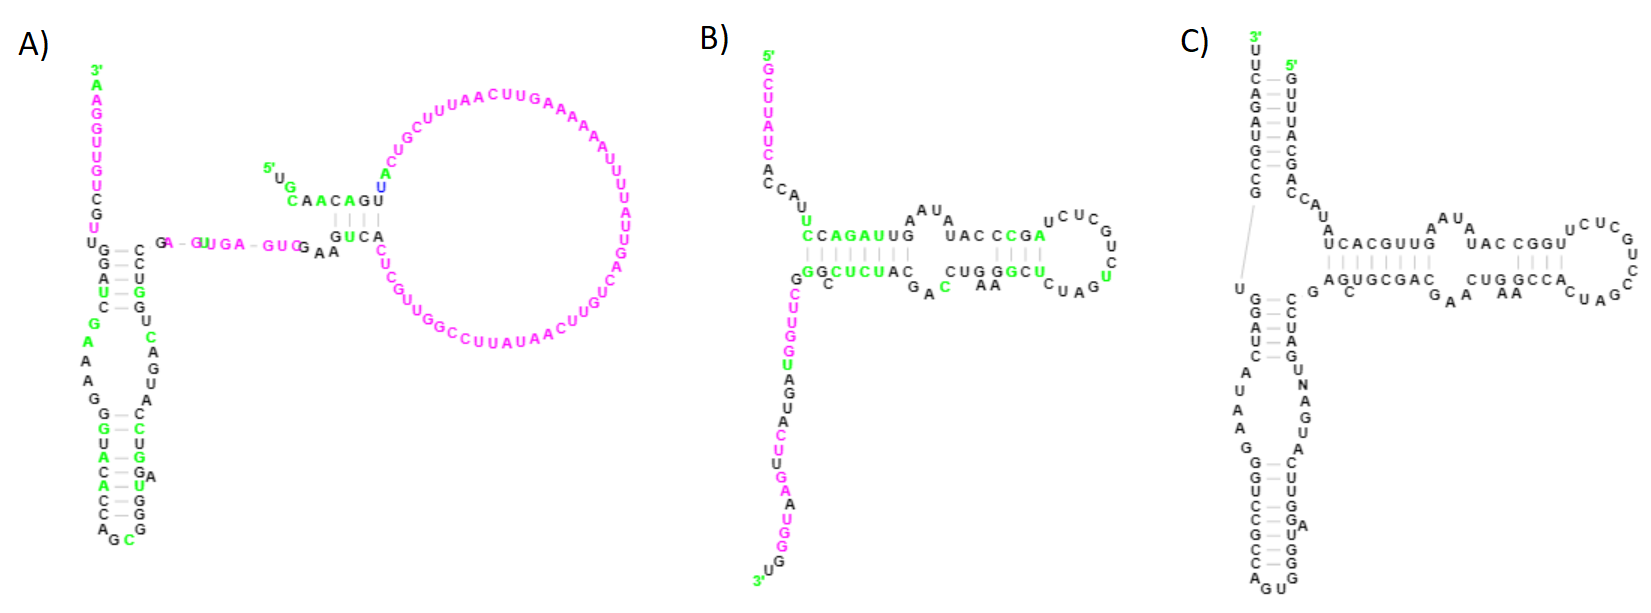
\includegraphics[width=140mm]{../img/kap02/intro/alignMotivationTemplate.png}
  \caption{Dvě sekundární RNA struktury s RNAcentral ID A) URS00006E712C, B)
  URS0000AB09C9 vygenerované nástrojem Traveler a C) vzorové sekundární RNA
  struktury d.5.e.S.oshimae.}
\end{figure}

Přidáním struktury, ze které jsou obě sturktury odvozené, je mnohem jasnější,
na která místa koukat pří hledání podobností a rozdílů. Přesto nemusí být
nějaká podobnost hned jasná, a proto jsme se zaměřili na způsoby, jak znázornít
mapování nukleotidů na vzorovou strukturu.

\section{Důsledek využívaní vzorové struktury}

Využívání vzorové struktury pro analýzu má zřejmý a důležitý důsledek. Náš
nástroj usnadňuje analýzu $N$ struktur, které byly vygenerované ze stejné
vzorové struktury. 

Protože Traveler umožňuje zadat, která vzorová struktura se má použít pro
generování je teoreticky možné, porovnávat jakékoliv dvě sekundární RNA
struktury, pokud bude jejich rozložení vygenerované na základě stejné vzorové
struktury. Pokud se ale pokusíme vygenerovat rozložení struktury pomocí vzorové
struktury, která je úplně jiná, nebude existovat žádná podobnost se vzorovou
strukturou, a tím pádem naše metody, které spoléhají na podobnost vzorové
struktury s vygenerovanou nebudou užitečné.

\section{Překládání struktur}

Vygenerované sekundární struktury jsou podobné vzorové struktuře, a tím pádem
bývají podobné i ostatním vygenerovaným strukturám ze stejné vzorové struktury.
Dává proto smysl se pokusit struktury přes sebe přeložit, aby se spojily
společné části a vynikly rozdíly. Pouhým přeložením podobných struktur přes
sebe však získáme výsledek, který neposkytuje příliš zajímavé informace a je
málo přehledný.

\begin{figure}[H]
  \centering
  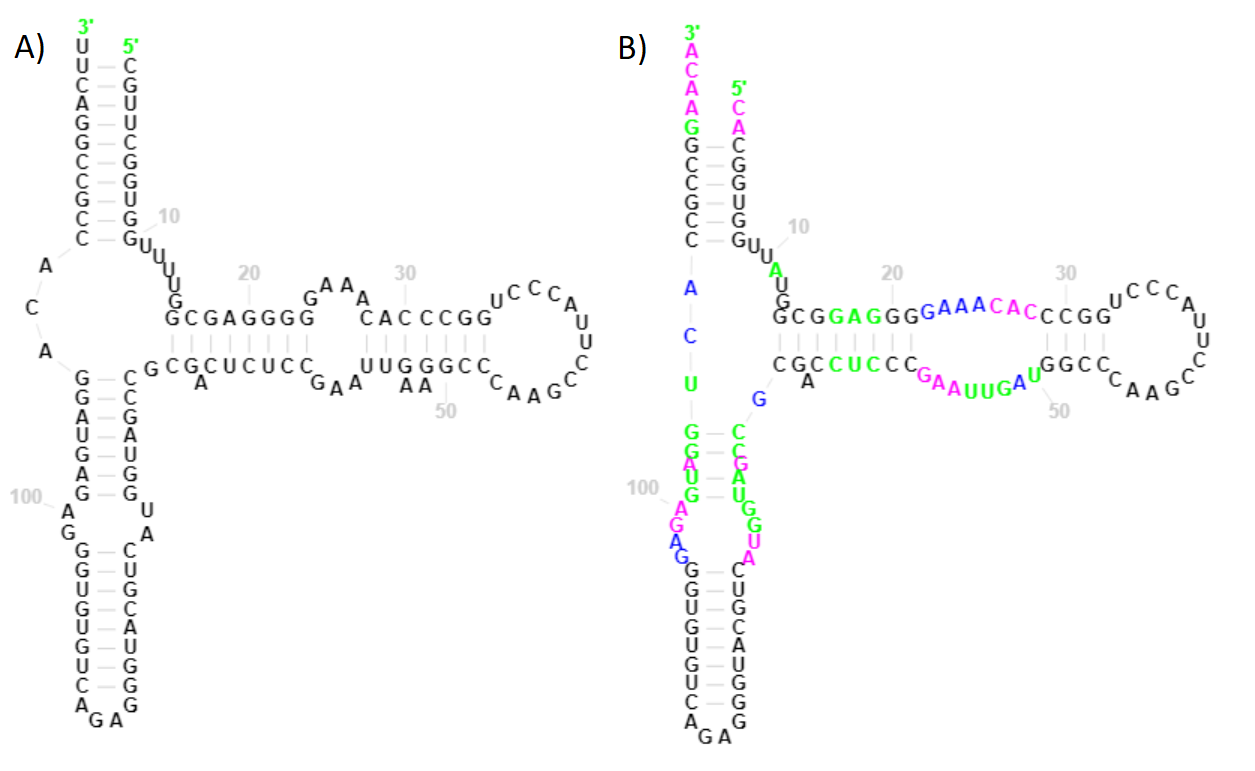
\includegraphics[width=140mm]{../img/kap02/align/structures.png}
  \caption{A) Struktura s RNAcentral ID URS00000B9D9D vygenerovaná nástrojem
  Traveler pomocí B) vzorové struktury d.5.b.A.madurae vedle sebe.}
\end{figure}

\begin{figure}[H]
  \centering
  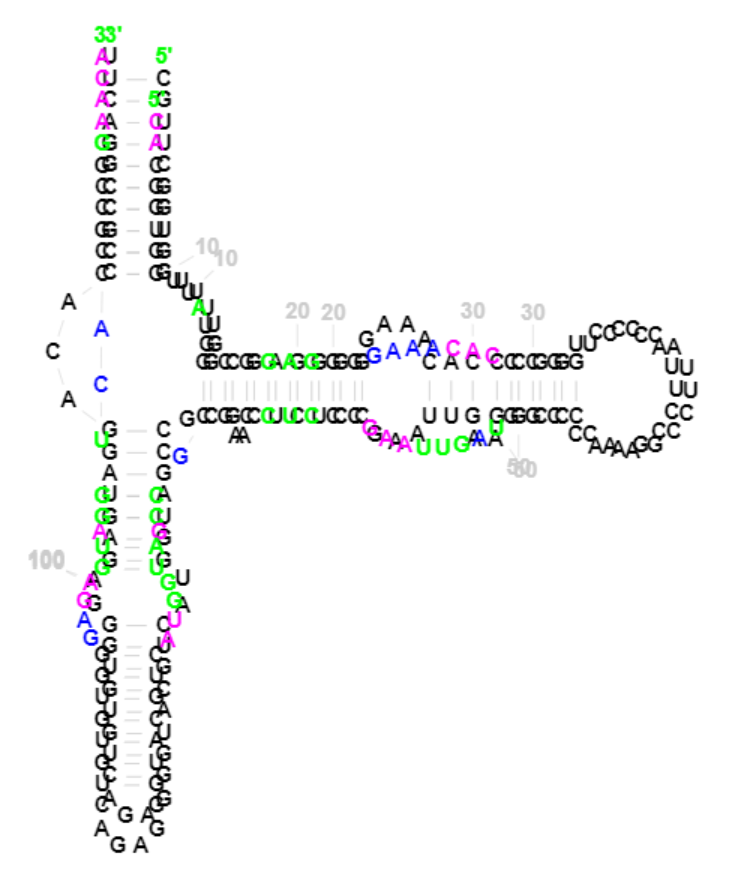
\includegraphics[height=90mm]{../img/kap02/align/unaligned.png}
  \caption{A) Struktura s RNAcentral ID URS00000B9D9D vygenerovaná nástrojem
  Traveler pomocí B) vzorové struktury d.5.b.A.madurae přeložené přes sebe.}
\end{figure}

\subsection{Zarovnání}

Je potřeba najít způsob, jak řešit problém přesunu a zarovnání struktury,
protože manuální manipulace pomocí přetažení myší nebo zadávání pozice může být
zbytečně obtížná, zejména pokud se snažíme dosáhnout přesného zarovnání. Proto
je velmi užitečné umožnit zarovnání sekundární RNA struktury na konkrétní
nukleotid nebo skupinu nukleotidů ze vzorové struktury. 

Pokud je vybrán vzorový nukleotid $v$ pro nukleotid $n$ z ostatních struktur,
jehož vzor je $v$, je celá struktura přesunuta tak, aby se nukleotidy $v$ a $n$
překrývaly. 

\subsubsection{Skupiny nukleotidů}

Pokud se snažíme najít větší skupinu nukleotidů, na které chceme strukturu
zarovnat, koukáme se na posunutí pro konkrétní nukleotidy a následně vybereme
buď posunutí které zarovná nejvíc nukleotidů nebo to které zarovná skupinu
nukleotidů které jsou v části struktury, která nás právě zajímá.

Pro hledání konkrétního posunutí pro zarovnání jsme použili naivní způsob,
který nezaručuje nejlepší možné zarovnání, ale zároveň je poměrně přímočarý a
dává rozumné výsledky, díky již zmíněné podobnosti struktur.

Postupně se prochází každá struktura. V první iteraci se porovná pozice každého
nukleotidu s pozicí ve vzorové struktuře. Na základě pozice se roztřídí
nukleotidy. Třídění funguje tak, že do stejné skupiny indexované posunutím se
přidají všechny vzorové nukleotidy, na které se struktura zarovná daným posunutím.
Na konci první iterace se skupiny, které jsou menší než $x$ odeberou.

V druhé iteraci se postupuje podobně, ale používají se poslední vytvořené
skupiny na filtrování, tím se snažíme docílit, zarovnání na stejné nukleotidy.
Filtrování pomocí skupin ingoruje všechny nukleotidy, jejiž vzor není v nějaké
skupině, pomocí které filtrujeme. Pokud během iterace nevzniknou žádné skupiny,
řeší se iterace daná iterace zvlášť bez filtrování.

\begin{figure}[H]
  \centering
  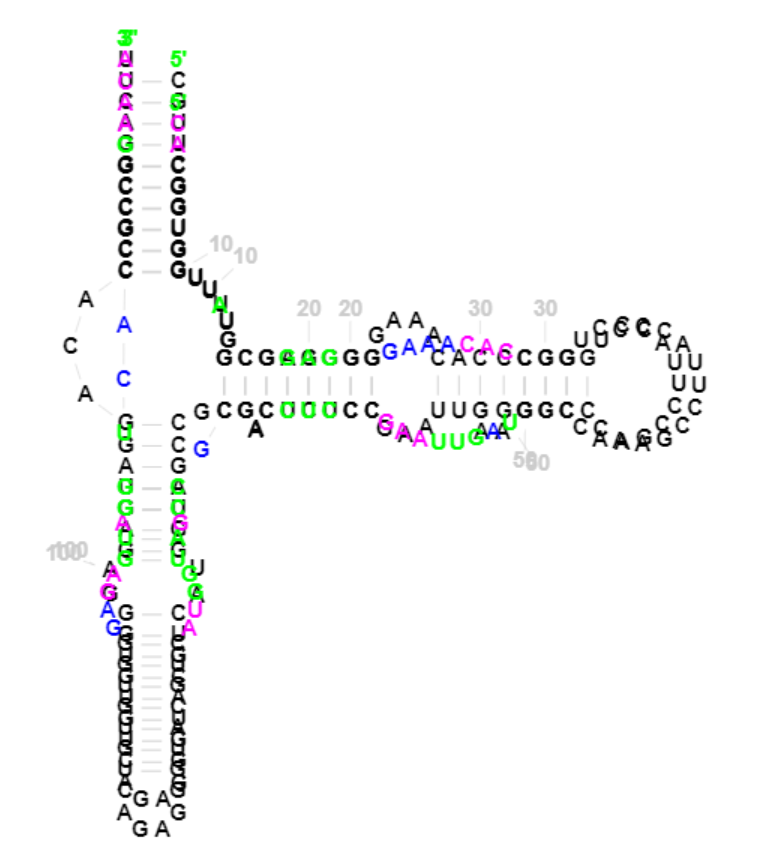
\includegraphics[height=90mm]{../img/kap02/align/alignedAlpha1.png}
  \caption{A) Struktura s RNAcentral ID URS00000B9D9D vygenerovaná nástrojem
  Traveler pomocí B) vzorové struktury d.5.b.A.madurae přeložené přes sebe a
  zarovnané.}
\end{figure}

\subsection{Průhlednost struktur}

V přeložených a zarovnaných strukturách nelze snadno rozeznat, které nukleotidy
jsou společné a překrývají se a které nejsou. Přidáním průhlednosti je možné
tuto situaci rozlišit, protože překrývající se nukleotidy budou mít sytější
barvu než ty, které se nepřekrývají.

\begin{figure}[H]
  \centering
  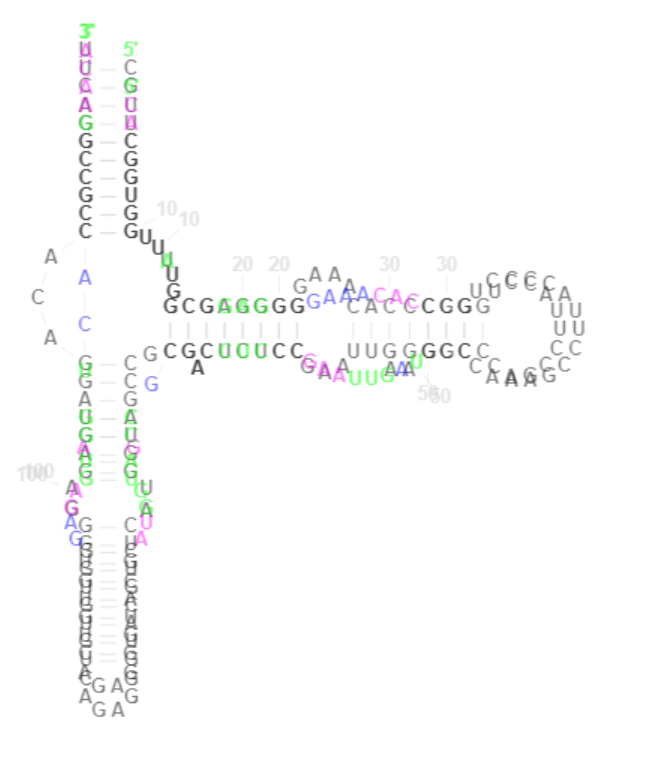
\includegraphics[height=90mm]{../img/kap02/align/aligned.png}
  \caption{A) Struktura s RNAcentral ID URS00000B9D9D vygenerovaná nástrojem
  Traveler pomocí B) vzorové struktury d.5.b.A.madurae přeložené přes sebe,
  zarovnané a s průhledností.}
\end{figure}

\subsection{Rozmazání struktur}

Zarovnávání struktur bohužel neřeší všechny výzvy. Výsledné obrázky se mohou
zdát rozmazané. To je způsobeno tím, že ačkoli má nukleotid vzorový nukleotid,
který je stejný, jeho pozice se může v rozložení mírně lišit v důsledku metody
generování dat. Tento fakt může způsobit, že popisky nukleotidů vypadají
rozmazaně.

Jako přímočaré řešení se může zdát posunoutí jednotlivých nukleotidů, které jsou
blízko sebe, aby dokonale překrývaly jejich vzory. Věříme, že by to vyřešilo
zmíněný problém bez významné deformace struktury.

\section{Obarvení struktur}

Vstupní data obsahují barevné označení nukleotidů. Slouží k lepšímu
zorientování se ve struktuře vzhledem ke vzorové struktuře. Jejich význam je
následující.

Černá barva značí, že nukleotid leží na poloze vzorového nukleotidu se stejným
názvem. Zelenou barvou jsou označený ty nukleotidy jejiž vzorový nukleotid bylo
třeba přejmenovat. Modrou barvou jsou vyznačený posunutý nukleotid. A poslední
růžovou barvu mají nově přidané nukleotidy.

\begin{figure}[H]
  \centering
  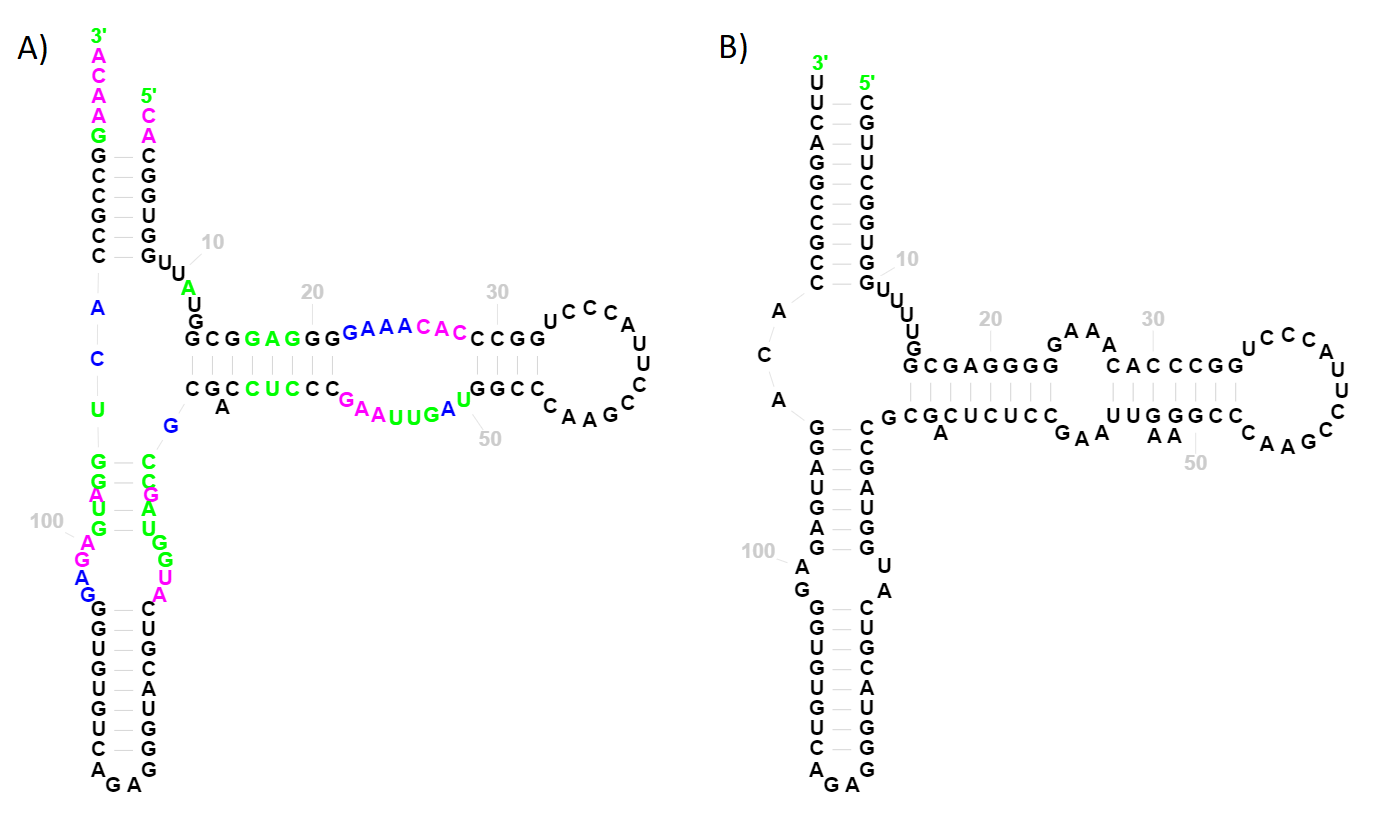
\includegraphics[width=140mm]{../img/kap03/inputDataColors.png}
  \caption{A) Struktura s RNAcentral ID URS00000B9D9D vygenerovaná nástrojem
  Traveler pomocí B) vzorové struktury d.5.b.A.madurae.}
\end{figure}

\section{Transformace na vzor}

Užitečnou metodou je transformace mezi vzorovou a cílovou strukturou. Každý
nukleotid, který má svůj vzorový nukleotid, se přemístí na pozici vzorového
nukleotidu a nukleotidy, které ve vzoru nejsou, jsou skryté. Tato metoda je
velmi užitečná pro práci s dvěma strukturami, které jsou si podobné, nebo pro
získání počátečního přehledu o tom, co je na co namapováno. 

Slabou stránkou této metody je její použití při práci s více než dvěma
strukturami nebo strukturami, které jsou velmi odlišné. V takových situacích se
na obrazovce děje mnoho věcí a je obtížné se soustředit a vypozorovat něco
užitečného.

\begin{figure}[H]
  \centering
  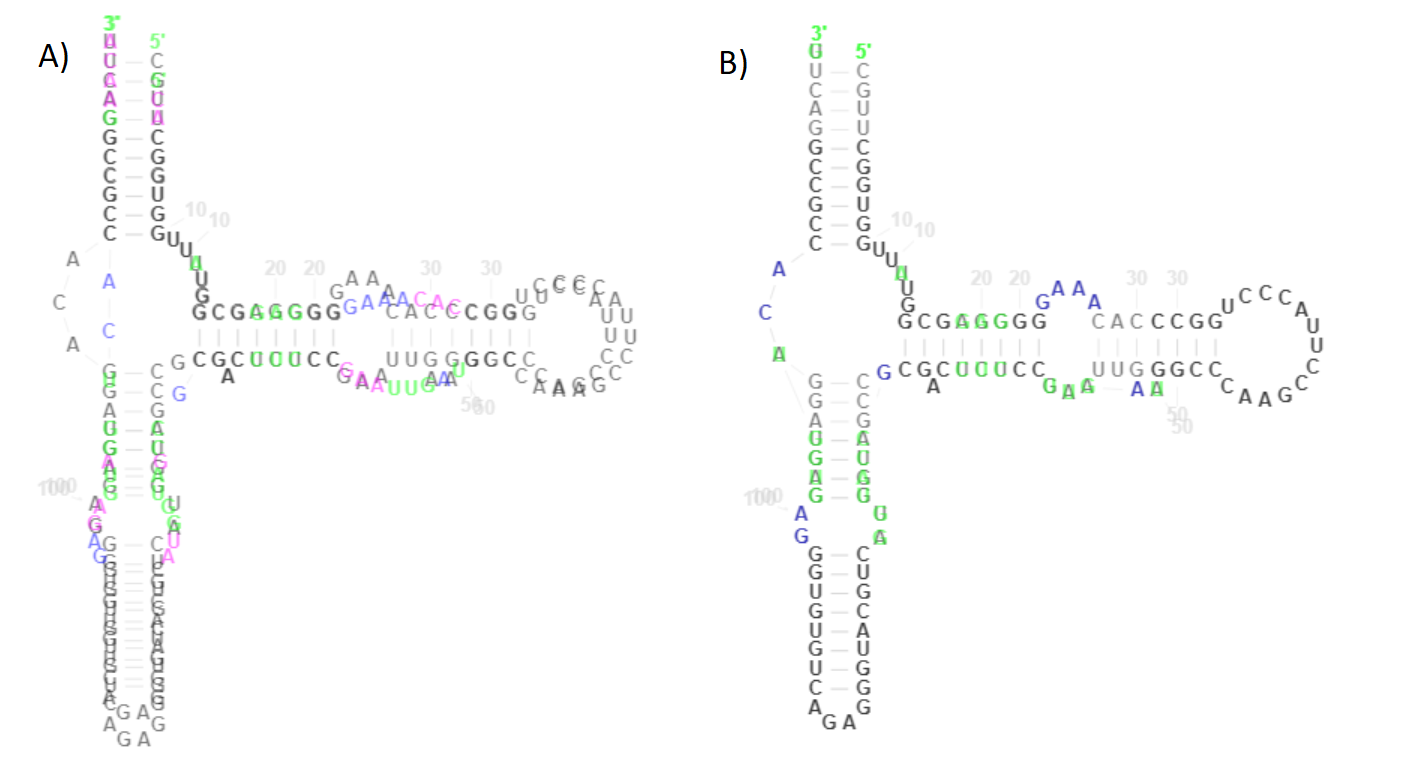
\includegraphics[width=140mm]{../img/kap02/animation.png}
  \caption{Struktura s RNAcentral ID URS00000B9D9D vygenerovaná nástrojem
  Traveler pomocí vzorové struktury d.5.b.A.madurae přeložené přes sebe A) před
  transformací a B) po transformaci.}
\end{figure}

\section{Mapovací čáry}

Vědomost o tom, který nukleotid se na co mapuje, může být důležitá pro odhalení
rozdílů a podobností mezi strukturami. V našem úsilí zprostředkovat tuto
informaci již před transformací na vzorovou sturkturu jsme přišli s čárami,
které spojují každý nukleotid s jeho vzorovým nukleotidem.

\begin{figure}[H]
  \centering
  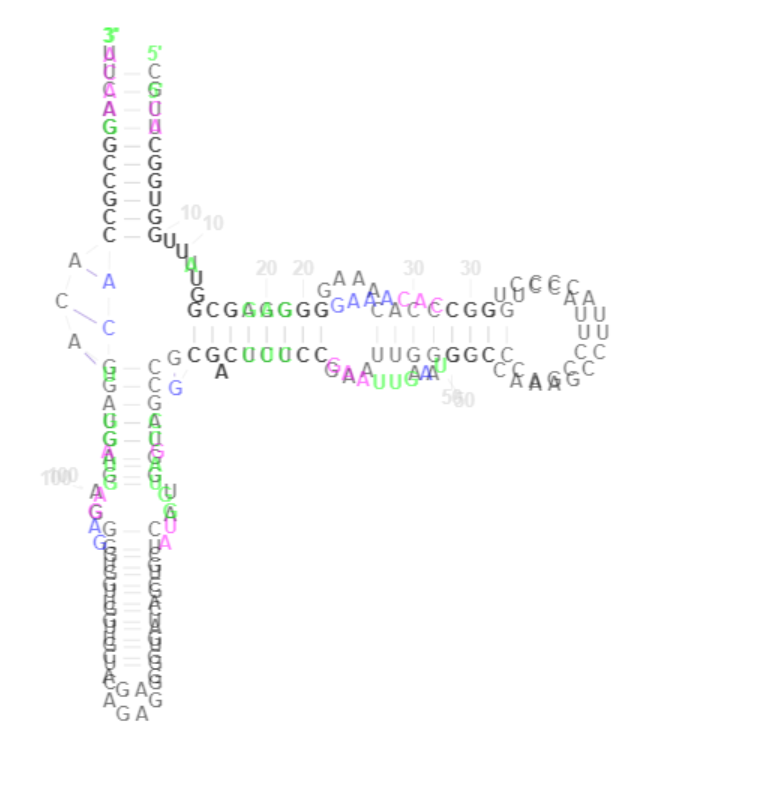
\includegraphics[height=90mm]{../img/kap02/mappingLines/small.png}
  \caption{Struktura s RNAcentral ID URS00000B9D9D vygenerovaná nástrojem
  Traveler pomocí vzorové struktury d.5.b.A.madurae přeložené přes sebe s
  mapovacíma čárama.}
\end{figure}

Bohužel tento způsob se zvětšující se velikostí struktury stáva velmi
nepřehledným, přesto si myslíme že můžou být užitečné.

\begin{figure}[H]
  \centering
  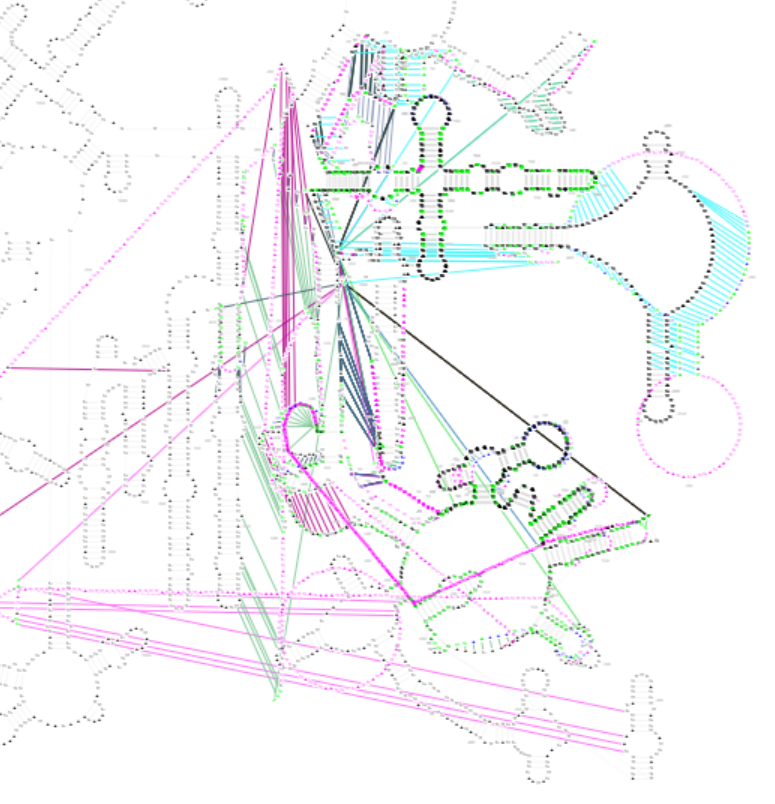
\includegraphics[height=100mm]{../img/kap02/mappingLines/big.png}
  \caption{Výřez z mnoha struktur vygenerovaných nástrojem Traveler pomocí vzorové struktury DD\_28S\_3D přeložených přes sebe s mapovacími čárami.
  Každá struktura má vlastní barvu mapovacích čar.}
\end{figure}

\section{Využití stromu}

V projektu Traveler byla použita stromová reprezentace pro sekundární RNA
strukturu, ve které je vnitřní vrchol, tedy má více jak jednu hranu, bázový pár
a listem, tedy má jednu nebo žádnou hranu, je nezpárovaný nukleotid. Strom pak
lze vytvořít následovně. První nepárové nukleotidy ze začátku a z konce přidáme
jako samostatné vrcholy. Potom jdeme postupně po bázových párech. První bázový
pár tvoří kořen. Další bázové páry připojujeme a tvoříme strom. Pokud narazíme
na nezpárovaný nukleotid přidáme ho jako list k poslednímu přidanému bázovému
páru. Větvení strukutry vyustí ve větvení stromu. 

\begin{figure}[H]
  \centering
  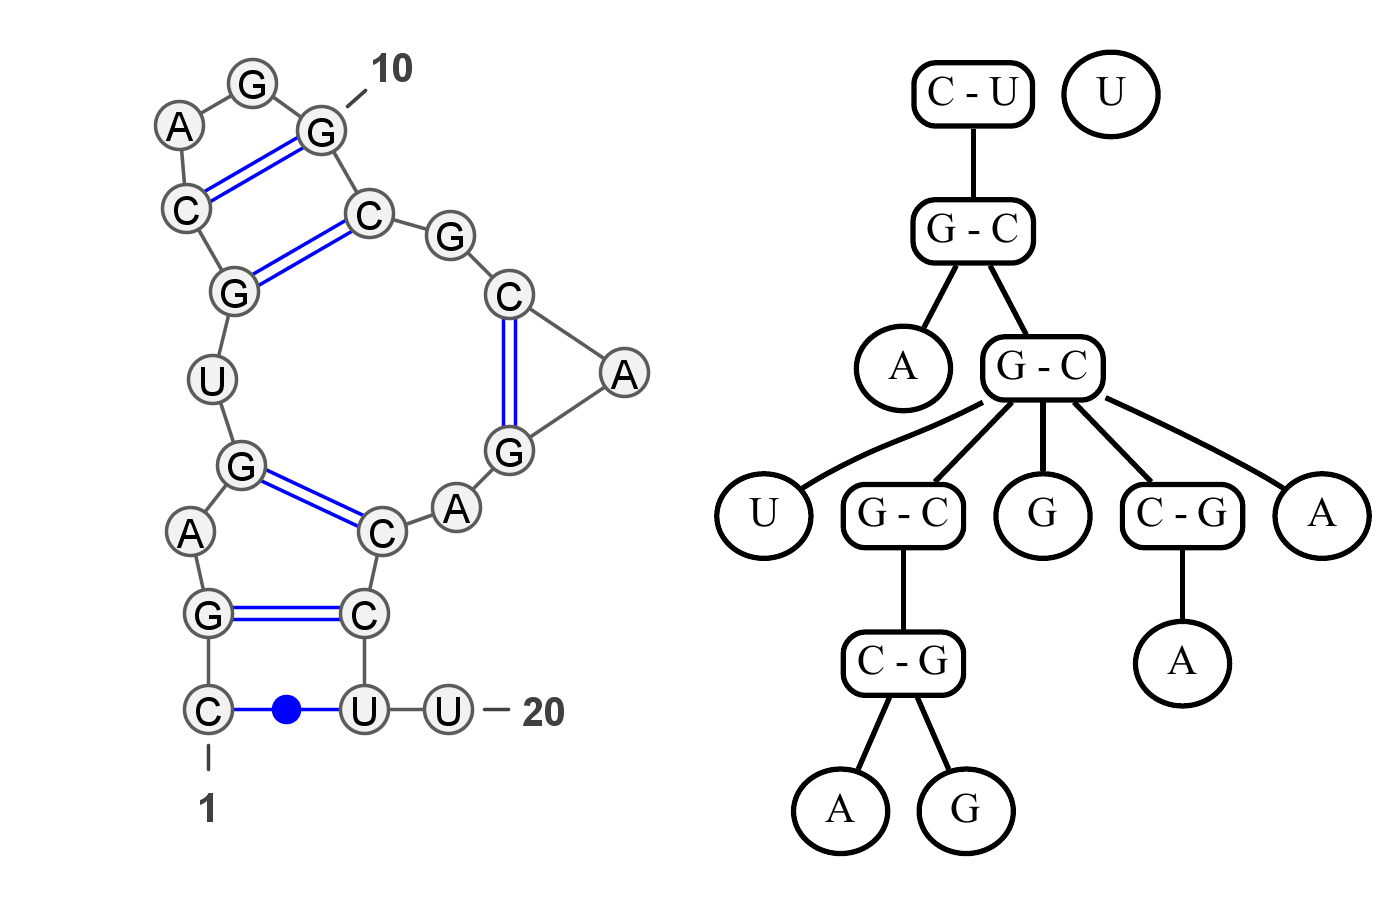
\includegraphics[width=140mm]{../img/kap02/tree/tree.png}
  \caption{Vlevo je uměle vytvořená struktura zobrazená nástrojem Varna. Vpravo je jeho stromová reprezentace.}
\end{figure}

Stromovu strukturu jsme neměli v úmyslu použít na nic konkrétního, ale chtěli
jsme prozkoumat možnosti lokálních transformací struktury pro dosažení
zarovnání více podobných částí, které jsou třeba jenom posunuté, jako je to
například v následující části dvou struktur, které jsou zarovnané dvouma
způsoby.

\begin{figure}[H]
  \centering
  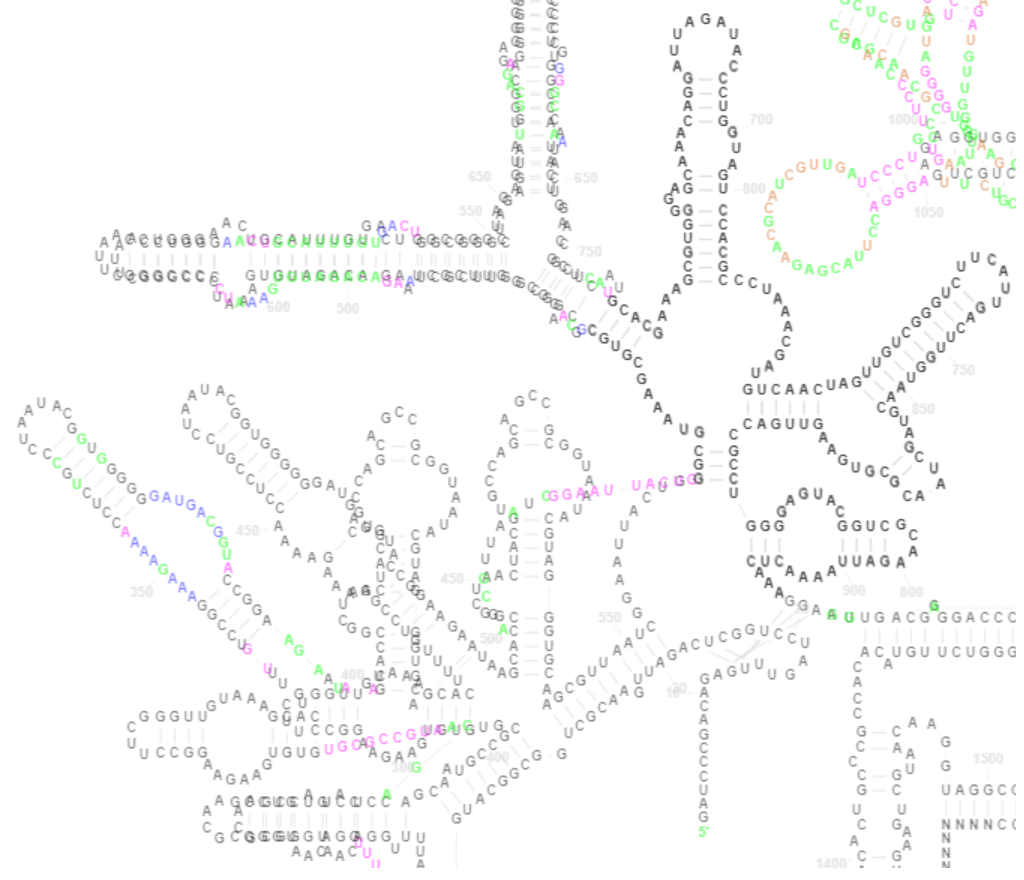
\includegraphics[height=100mm]{../img/kap02/tree/align1.png}
  \caption{První způsob zarovnání.}
\end{figure}

\begin{figure}[H]
  \centering
  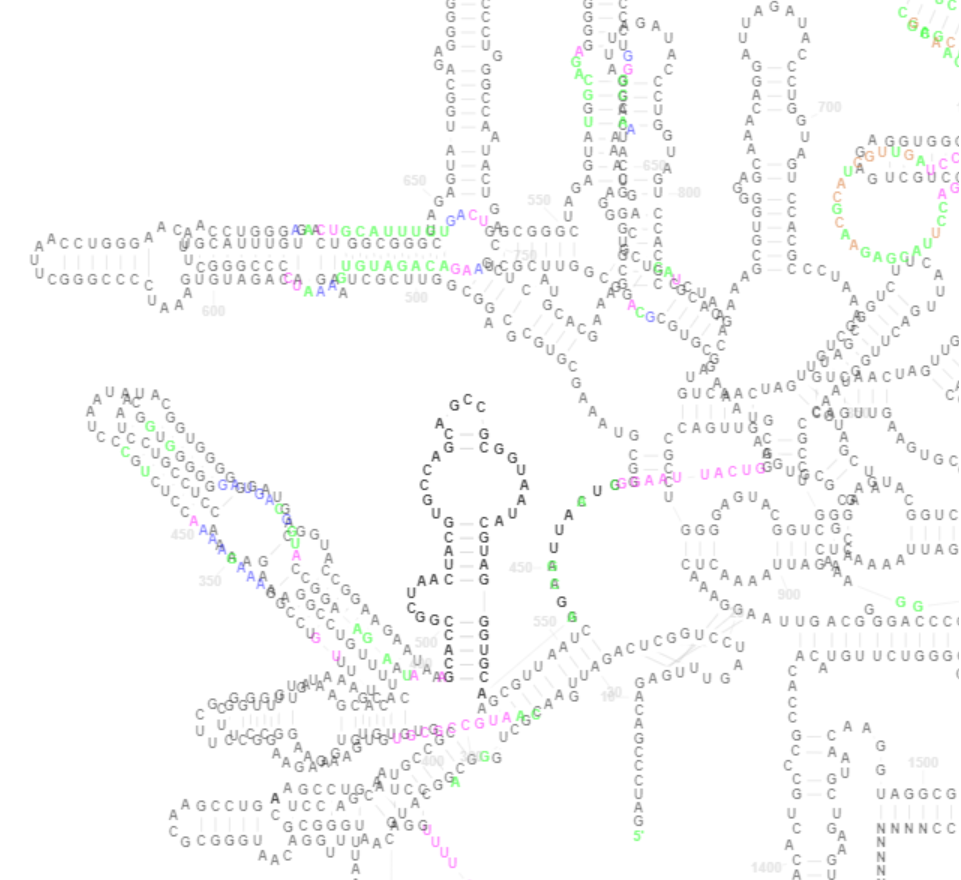
\includegraphics[height=100mm]{../img/kap02/tree/align2.png}
  \caption{Druhý způsob zarovnání.}
\end{figure}

Po zvážení jsme dospěli k názoru, že není možné provést úpravu struktury, která
by významně nedeformovala strukturu. Jakákoli úprava části struktury znamená
posunutí nějakého zbytku struktury, což může zasáhnout do jiné části. Proto by
bylo nezbytné odebrat některé nukleotidy. Ty, které nejvíce překážejí, jsou ty
přidané. Pokud bychom odebrali tyto přidané nukleotidy, dostali bychom se na
stejný výsledek jako s transformací struktury na vzorovou strukturu.

\section{Zvolené metody}

Naše knihovna přímo podporuje překládání a zarovnání struktur na konkrétní
nukleotid nebo skupinu nukleotidů bez zarovnání na úrovni jednotlivých
nukletidů pro odstranění rozmazání struktur. Lze transformovat struktury na
vzorovou strukturu a upravovat průhlednost struktur.


\chapter{Programátorská dokumentace}

\section{Volba technologií}

\subsection{Programovací jazyk}

Volba programovacího jazyka byla poměrně přímočará. Chtěli jsme napsat
knihovnu, která se bude používat na webu.
Javascript\footnote{https://developer.mozilla.org/en-US/docs/Web/JavaScript} je
v tomto případě jasnou volbou, protože to je v podstatě to jediné, co se
používá. Přesto Javascript není jazyk, ve kterým je naše knihovna psaná,
protože se jedná o dynamicky typovaný jazyk, což s sebou nese určité výhody pro
jednoduché a rychlé psaní kódu, ale u větších projektů se to stává nevýhodou.
Naše knihovna je napsaná v
Typescriptu\footnote{https://www.typescriptlang.org/}, což je nadmnožina
Javascriptu, snažící se řešit jeho slabiny a navíc ho lze snadno přeložit do
Javasrciptu a v této formě distribuovat. Při tomto překladu je možné zachovat i
informaci o konkrétních typech, tím pádem projekty, využívající naší knihovnu,
psané v Typescriptu nejsou ochuzené o typovou kontrolu, kterou typescript
nabízí.

\subsection{Překlad jazyka}

\subsection{verzování}

Pro verzování používáme Git a celou repository hostujeme na GitHubu. Jediným
důvodem pro toto rozhodnutí, že obě technologie známe, nemáme s nimi problém a
neviděli jsme důvod hledat jiné možnosti.

\subsection{Knihovna D3.js}

D3.js\footnote{https://d3js.org/} je knihovna v jayzce Javascript pomáhající
přivést data k životu využívající především
SVG\footnote{https://developer.mozilla.org/en-US/docs/Web/SVG} formát, se
kterým se dá v
HTML\footnote{https://developer.mozilla.org/en-US/docs/Learn/Getting_started_with_the_web/HTML_basics}
pohodlně pracovat. Její důraz na webové standardy dává uživateli možnost
využívat moderní prohlížeče naplno bez dalších frameworků. S knihovnou není
nejjednodušší se naučit pracovat, ale nabízí minimální overhead a její velkou
předností je rychlost.

\subsection{SVG nebo canvas}

V počátcích jsme chtěli k zobrazování používat SVG. Jedná se o webový standard,
který lze skvěle kombinovat s ostatními standardy jako je
CSS\footnote{https://developer.mozilla.org/en-US/docs/Web/CSS},
DOM\footnote{https://developer.mozilla.org/en-US/docs/Web/API/Document_Object_Model},
Javascript. V kombinací s D3.js knihovnou je pak dělání animací nebo
aktualizaci stavu SVG objektů jednoduché.

Nebyl důvod SVG nevyužívat, ale později jsme na vlastní kůži pocítili slabinu
SVG. SVG se při vykreslování tisícovek objektů stává velmi pomalé. Takového
počtu objektů můžeme dosáhnout pouze s jednou sekundární RNA strukturou, my
navíc chceme zobrazit více takových struktur a ještě s nimi dynamicky pracovat. 

Tím se pro nás stalo SVG nepoužitelné. Další možností bylo využití
canvasu\footnote{https://developer.mozilla.org/en-US/docs/Web/API/Canvas_API},
který slibuje výrazně lepší výkon a lze ho stále jednoduše používat.

Některé pro nás klíčové funkce D3.js knihovny lze využít i pro práci s
canvasem. Konkrétně se jedná o zoom, panning a animace.

U canvasu jsme nakonec i zůstali, přestože při práci s desítkama velkých
struktur vykreslování není plynulé.

\section{Vstupní data}

Jak jsme již zmiňovali, naše knihovna využívá výstupní data nástroje Traveler
jako vstupní data. Jedná se o data ve formátu JSON, obsahující všechny potřebné
informace o rozložení nukleotidů, jejich párování, velikostech popisků, barvách
a tlouštkách čar. Kromě informací o rozložení obsahuje také informace o
potřebných editacích vzorové sekundární struktury.

V rámci R2DT projektu vzníká i JSON
schéma\footnote{https://github.com/LDWLab/RNA2D-data-schema}, které by mělo
popisovat strukturu vstupních dat. Schéma je stále ve vývoji, proto aktuální
výstupy R2DT nebo Traveleru neodpovídájí schématu a je dost možné, že se jejich
výstupy budou v budoucnu měnit a naše knihovna se jim bude přizpůsobovat,
\red{TODO: přepsat}protože RNAcentral, využívající R2DT, je největší databází s
2D RNA strukturama.

Samotná struktura dat není složitá, ale popíšeme zde pouze tu část, kterou
aktuálně využíváme, kromě toho, že ostatní data pro nás nejsou duležitá, tak
jak již bylo zmíněno samotná struktura dat není pevně daná a může se měnit.

Jedná se o objekt, který má dvě položky - \texttt{classes}, což je pole objektů
popisující třídy říkající způsob zobrazení struktury, podobně jako to kaskádové
styly (CSS) diktují pro webové stránky a \texttt{rnaComplexes}. 

\texttt{rnaComplexes} je pole polí sloužící pro popis celých skupin RNA
struktur. Naše knihovna pracuje vždy pouze s nultým prvkem. Neviděli jsme důvod
to dělat jinak, a pokud by se nějaký důvod našel v budoucnu, neměl by být
problém naší knihovnu přizpůsobit situaci (např. rozšířením o novou metodu pro
zachování zpětné kompatibility).

V rámci naší knihovny jsme vytvořili interface, který vstupní data musí
splňovat. Struktura zbytku dat by měla být jasně viditelná z následujícího
UML\footnote{https://www.uml.org/} diagramu těchto interfaceů.

\begin{figure}[H]
  \centering
  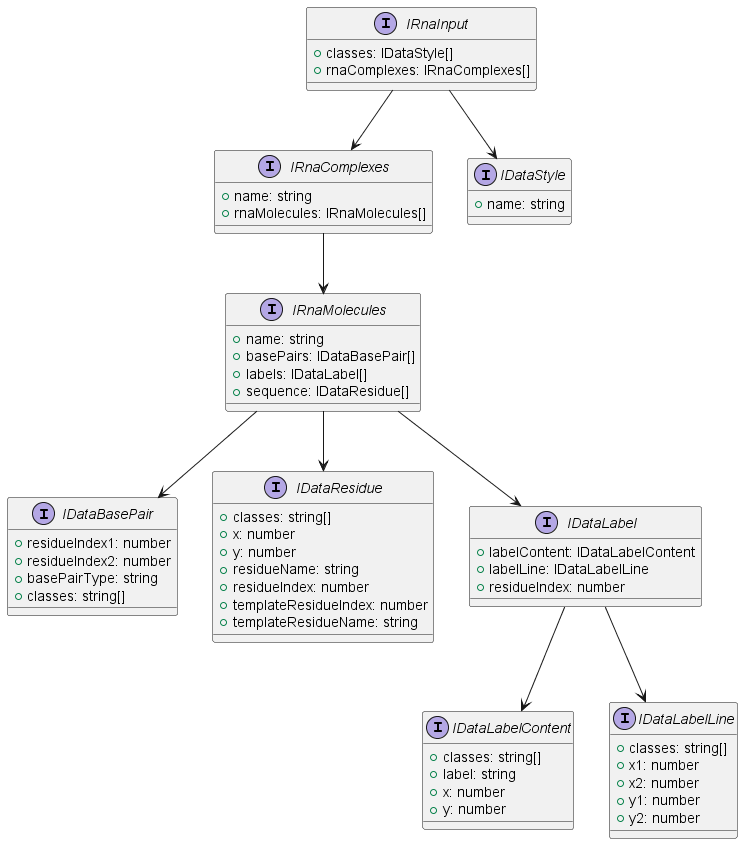
\includegraphics[width=145mm]{../img/rnaInput.png}
  \caption{Interface pro vstupní data}
\end{figure}

Při vykreslení dat si můžeme všimnout různého obarvení jednotlivých residue.
Tyto barvy slouží k lepšímu zorientování ve struktuře vzhledem ke vzorové
struktuře. Černá barva značí, že residue leží na poloze vzorového residue se
stejným názvem. Zelenou barvou jsou označený ty residue jejiž vzorový residue
bylo třeba přejmenovat. Modrou barvou jsou vyznačený posunutý residue. A poslední
růžovou barvu mají nově přidaný residue.

\begin{figure}[H]
  \centering
  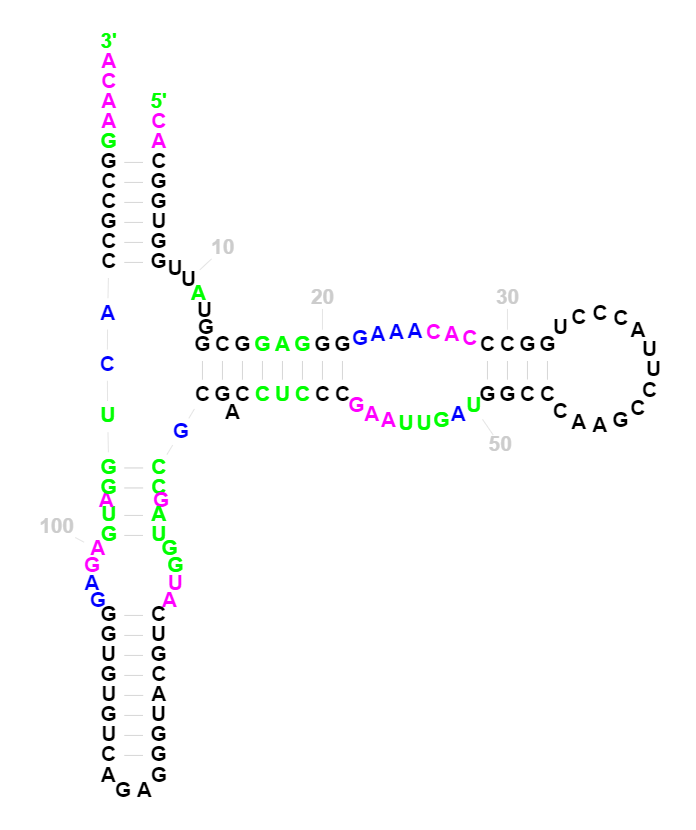
\includegraphics[width=145mm]{../img/inputDataColors.png}
  \caption{Odvozená sekundární RNA struktura URS00000B9D9D_471852 od d.5.b.A.madurae}
\end{figure}

\begin{figure}[H]
  \centering
  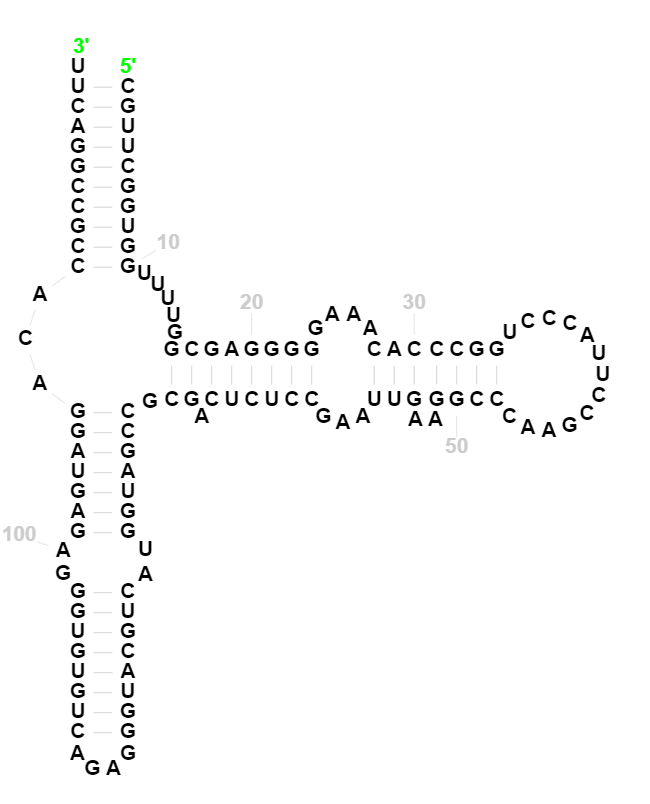
\includegraphics[width=145mm]{../img/inputDataTemplate.png}
  \caption{Vzorová sekundární RNA struktura d.5.b.A.madurae}
\end{figure}


\section{Objektový návrh}

\begin{figure}[H]
  \centering
  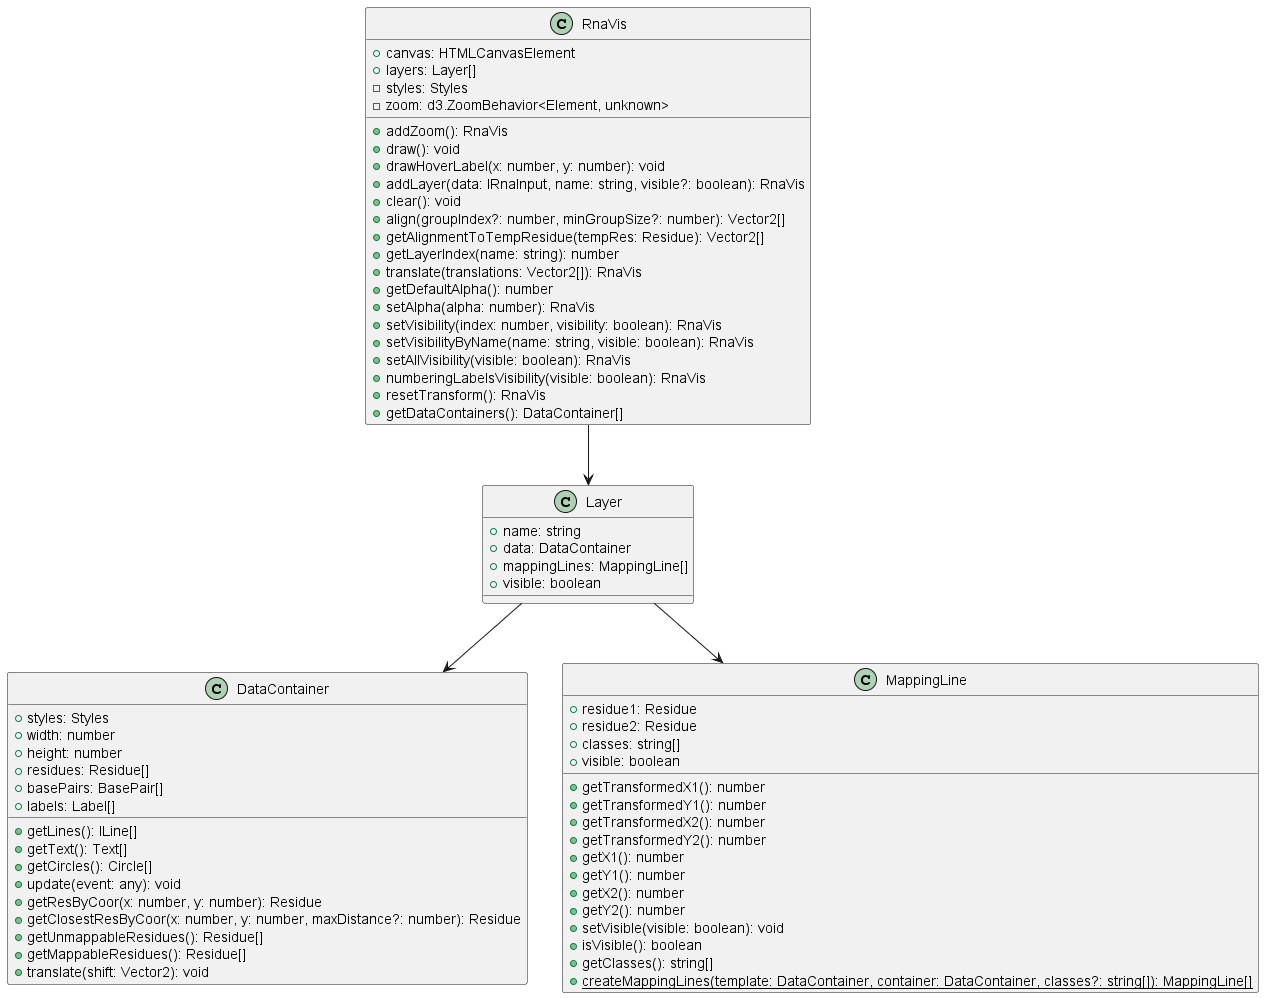
\includegraphics[width=145mm]{../img/rnaVis.png}
  \caption{Interface pro vstupní data}
\end{figure}

\begin{figure}[H]
  \centering
  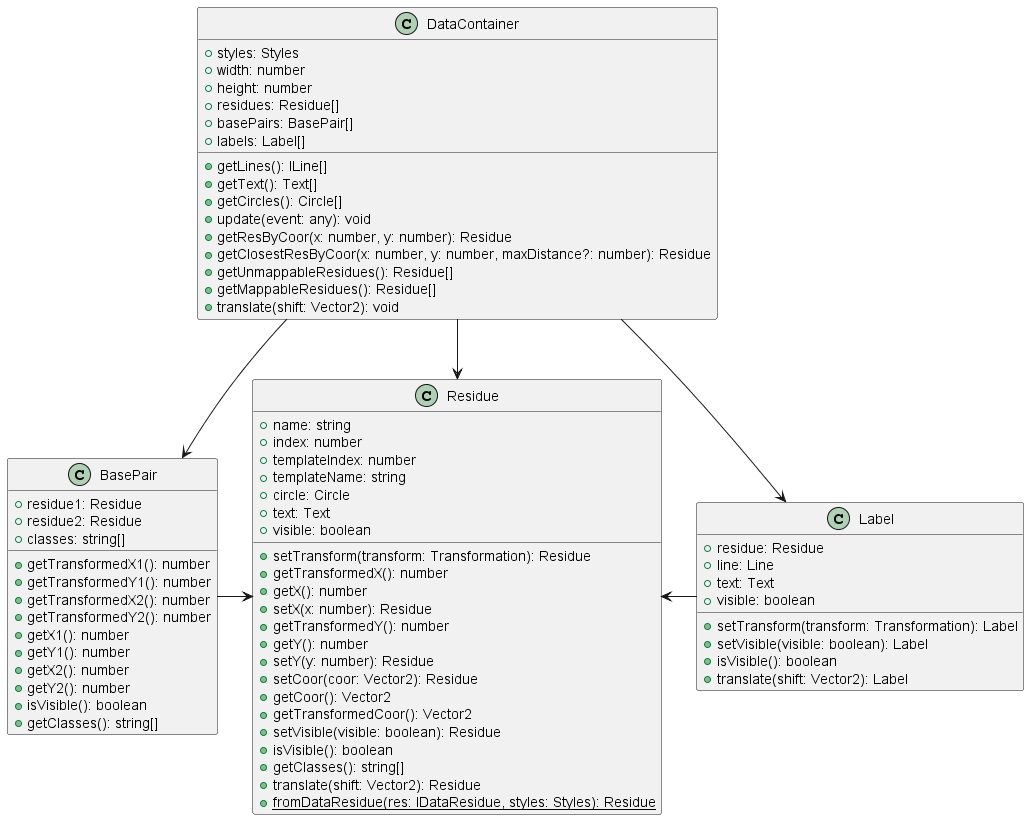
\includegraphics[width=145mm]{../img/dataContainer.png}
  \caption{Interface pro vstupní data}
\end{figure}

\begin{figure}[H]
  \centering
  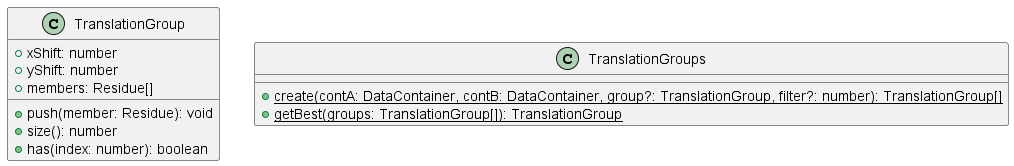
\includegraphics[width=145mm]{../img/translationGroups.png}
  \caption{Interface pro vstupní translationGroups}
\end{figure}

\begin{figure}[H]
  \centering
  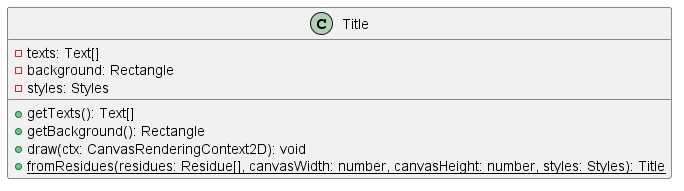
\includegraphics[width=145mm]{../img/title.png}
  \caption{Interface pro vstupní data}
\end{figure}

\begin{figure}[H]
  \centering
  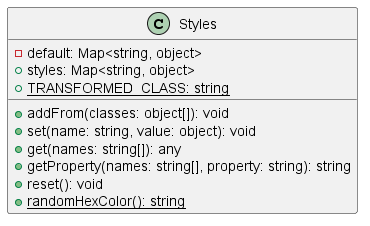
\includegraphics[width=145mm]{../img/styles.png}
  \caption{Interface pro vstupní data}
\end{figure}

\begin{figure}[H]
  \centering
  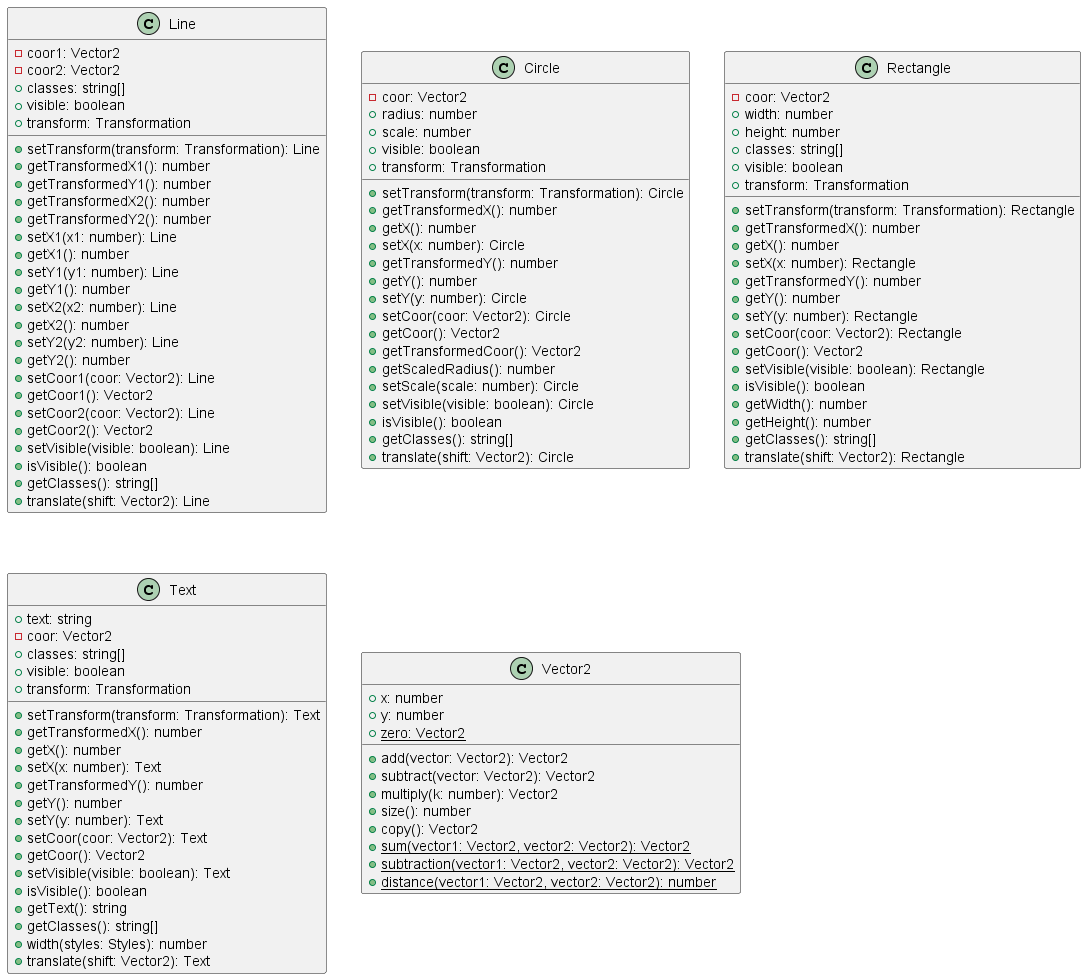
\includegraphics[width=145mm]{../img/primitives.png}
  \caption{Interface pro vstupní data}
\end{figure}

\begin{figure}[H]
  \centering
  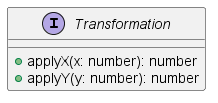
\includegraphics[width=145mm]{../img/iTransformation.png}
  \caption{Interface pro vstupní data}
\end{figure}

\begin{figure}[H]
  \centering
  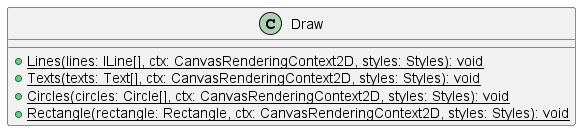
\includegraphics[width=145mm]{../img/draw.png}
  \caption{Interface pro vstupní data}
\end{figure}

\begin{figure}[H]
  \centering
  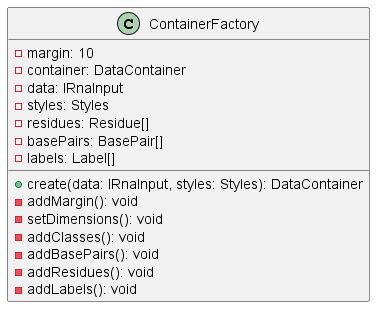
\includegraphics[width=145mm]{../img/containerFactory.png}
  \caption{Interface pro vstupní data}
\end{figure}

\begin{figure}[H]
  \centering
  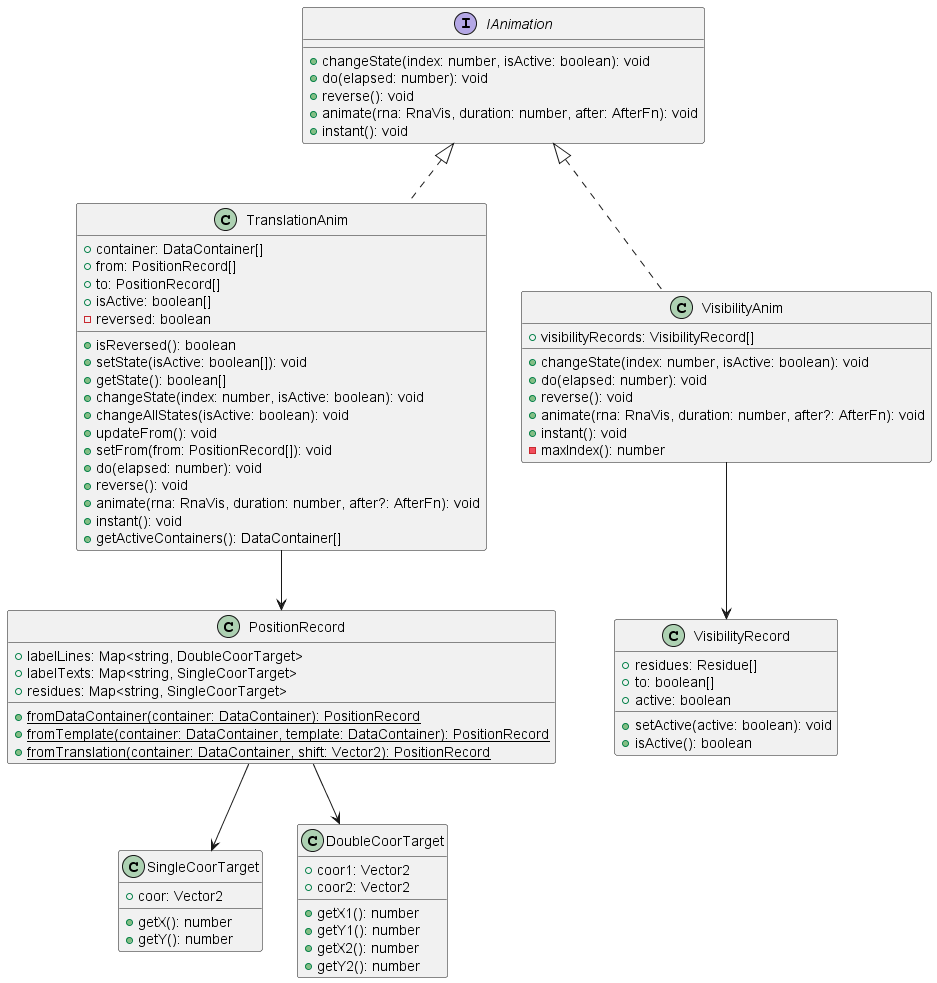
\includegraphics[width=145mm]{../img/animations.png}
  \caption{Interface pro vstupní data}
\end{figure}



%%% Fiktivní kapitola s instrukcemi k PDF/A

\chapter{Formát PDF/A}

Opatření rektora č. 13/2017 určuje, že elektronická podoba závěrečných
prací musí být odevzdávána ve formátu PDF/A úrovně 1a nebo 2u. To jsou
profily formátu PDF určující, jaké vlastnosti PDF je povoleno používat,
aby byly dokumenty vhodné k~dlouhodobé archivaci a dalšímu automatickému
zpracování. Dále se budeme zabývat úrovní 2u, kterou sázíme \TeX{}em.

Mezi nejdůležitější požadavky PDF/A-2u patří:

\begin{itemize}

\item Všechny fonty musí být zabudovány uvnitř dokumentu. Nejsou přípustné
odkazy na externí fonty (ani na \uv{systémové}, jako je Helvetica nebo Times).

\item Fonty musí obsahovat tabulku ToUnicode, která definuje převod z~kódování
znaků použitého uvnitř fontu to Unicode. Díky tomu je možné z~dokumentu
spolehlivě extrahovat text.

\item Dokument musí obsahovat metadata ve formátu XMP a je-li barevný,
pak také formální specifikaci barevného prostoru.

\end{itemize}

Tato šablona používá balíček {\tt pdfx,} který umí \LaTeX{} nastavit tak,
aby požadavky PDF/A splňoval. Metadata v~XMP se generují automaticky podle
informací v~souboru {\tt prace.xmpdata} (na vygenerovaný soubor se můžete
podívat v~{\tt pdfa.xmpi}).

Validitu PDF/A můžete zkontrolovat pomocí nástroje VeraPDF, který je
k~dispozici na \url{http://verapdf.org/}.

Pokud soubor nebude validní, mezi obvyklé příčiny patří používání méně
obvyklých fontů (které se vkládají pouze v~bitmapové podobě a/nebo bez
unicodových tabulek) a vkládání obrázků v~PDF, které samy o~sobě standard
PDF/A nesplňují.

Další postřehy o~práci s~PDF/A najdete na \url{http://mj.ucw.cz/vyuka/bc/pdfaq.html}.


\chapter*{Závěr}
\addcontentsline{toc}{chapter}{Závěr}


%%% Seznam použité literatury
%%% Seznam použité literatury (bibliografie)
%%%
%%% Pro vytváření bibliografie používáme bibTeX. Ten zpracovává
%%% citace v textu (např. makro \cite{...}) a vyhledává k nim literaturu
%%% v souboru literatura.bib.
%%%
%%% Příkaz \bibliographystyle určuje, jakým stylem budou citovány odkazy
%%% v textu. V závorce je název zvoleného souboru .bst. Styly plainnat
%%% a unsrt jsou standardní součástí latexových distribucí. Styl czplainnat
%%% je dodáván s touto šablonou a bibTeX ho hledá v aktuálním adresáři.

\bibliographystyle{czplainnat}    %% Autor (rok) s českými spojkami
% \bibliographystyle{plainnat}    %% Autor (rok) s anglickými spojkami
% \bibliographystyle{unsrt}       %% [číslo]

\renewcommand{\bibname}{Seznam použité literatury}

%%% Vytvoření seznamu literatury. Pozor, pokud jste necitovali ani jednu
%%% položku, seznam se automaticky vynechá.

\bibliography{literatura}

%%% Kdybyste chtěli bibliografii vytvářet ručně (bez bibTeXu), lze to udělat
%%% následovně. V takovém případě se řiďte normou ISO 690 a zvyklostmi v oboru.

% \begin{thebibliography}{99}
%
% \bibitem{lamport94}
%   {\sc Lamport,} Leslie.
%   \emph{\LaTeX: A Document Preparation System}.
%   2. vydání.
%   Massachusetts: Addison Wesley, 1994.
%   ISBN 0-201-52983-1.
%
% \end{thebibliography}


%%% Obrázky v bakalářské práci
%%% (pokud jich je malé množství, obvykle není třeba seznam uvádět)
\listoffigures

%%% Tabulky v bakalářské práci (opět nemusí být nutné uvádět)
%%% U matematických prací může být lepší přemístit seznam tabulek na začátek práce.
\listoftables

%%% Použité zkratky v bakalářské práci (opět nemusí být nutné uvádět)
%%% U matematických prací může být lepší přemístit seznam zkratek na začátek práce.
\chapwithtoc{Seznam použitých zkratek}

%%% Přílohy k bakalářské práci, existují-li. Každá příloha musí být alespoň jednou
%%% odkazována z vlastního textu práce. Přílohy se číslují.
%%%
%%% Do tištěné verze se spíše hodí přílohy, které lze číst a prohlížet (dodatečné
%%% tabulky a grafy, různé textové doplňky, ukázky výstupů z počítačových programů,
%%% apod.). Do elektronické verze se hodí přílohy, které budou spíše používány
%%% v elektronické podobě než čteny (zdrojové kódy programů, datové soubory,
%%% interaktivní grafy apod.). Elektronické přílohy se nahrávají do SISu a lze
%%% je také do práce vložit na CD/DVD. Povolené formáty souborů specifikuje
%%% opatření rektora č. 72/2017.
\appendix
\chapter{Přílohy}

\section{První příloha}

\openright
\end{document}
